    \documentclass[12pt,final,fleqn]{article}

% basic packages
\usepackage[margin=1in] { geometry }
\usepackage{amssymb,amsmath, bm}
\usepackage{verbatim}
\usepackage[latin1]{inputenc}
%\usepackage[OT1]{fontenc}
\usepackage{setspace}
\usepackage{enumitem}
\usepackage[bottom]{footmisc}
\usepackage{url}
\usepackage[font={bf}]{caption}
\usepackage{float}
%\usepackage{pgfplots}
%\usepackage[font={bf}]{caption}
\usepackage{setspace}
\usepackage{latexsym}
%\usepackage{euscript}
\usepackage{graphicx}
\usepackage{marvosym}
\usepackage{amsmath} 
\usepackage{authblk}
\usepackage{xcolor}
\usepackage{blindtext}
%\usepackage[varg]{txfonts}  Older version of ``g'' in math.

% Footnote double spacing and font size for journal submission
%\usepackage{footmisc}
%\setlength{\footnotesep}{\baselineskip}
%\renewcommand{\footnotelayout}{\normalsize\doublespacing}

% bibliography packages
\usepackage[natbibapa]{apacite}
\bibliographystyle{apsr}
\bibpunct{(}{)}{;}{a}{}{,}
\renewcommand{\bibname}{References}

% packages for tables
\usepackage{longtable}
\usepackage{booktabs, threeparttable}
\usepackage{threeparttablex}
%\usepackage{tabularx}
% dcolumn package
\usepackage{dcolumn}
\newcolumntype{.}{D{.}{.}{-1}}
\newcolumntype{d}[1]{D{.}{.}{#1}}
\captionsetup{belowskip=10pt,aboveskip=-5pt}
\usepackage{multirow}
% rotating package
\usepackage[figuresright]{rotating}
\usepackage{pdflscape}
\usepackage{subcaption}

% packages for figures
\usepackage{grffile}
\usepackage{afterpage}
\usepackage{float}
\usepackage[section]{placeins}


% theorem package
\usepackage{theorem}
\theoremstyle{plain}
\theoremheaderfont{\scshape}
\newtheorem{theorem}{Theorem}
\newtheorem{algorithm}{Algorithm}
\newtheorem{assumption}{Assumption}
\newtheorem{lemma}{Lemma}
\newtheorem{proposition}{Proposition}
\newtheorem{remark}{Remark}
\newcommand{\qed}{\hfill \ensuremath{\Box}}
\newcommand\indep{\protect\mathpalette{\protect\independenT}{\perp}}
\DeclareMathOperator{\sgn}{sgn}
\DeclareMathOperator{\tr}{tr}
\DeclareMathOperator{\argmin}{arg\min}
\DeclareMathOperator{\argmax}{arg\max}
\def\independenT#1#2{\mathrel{\rlap{$#1#2$}\mkern2mu{#1#2}}}
\providecommand{\norm}[1]{\lVert#1\rVert}
\renewcommand\r{\right}
\renewcommand\l{\left}
\newcommand\E{\mathbb{E}}
\newcommand\dist{\buildrel\rm d\over\sim}
\newcommand\iid{\stackrel{\rm i.i.d.}{\sim}}
\newcommand\ind{\stackrel{\rm indep.}{\sim}}
\newcommand\cov{{\rm Cov}}
\newcommand\var{{\rm Var}}
\newcommand\SD{{\rm SD}}
\newcommand\bone{\mathbf{1}}
\newcommand\bzero{\mathbf{0}}

% dotted lines in tables
%\usepackage{arydshln}

\usepackage{pdflscape}

% spacing between sections and subsections
\usepackage[compact]{titlesec}

% times new roman
%\usepackage{times}

% appendix settings
\usepackage[toc,page,header]{appendix}
\renewcommand{\appendixpagename}{\centering Appendices}
\usepackage{chngcntr}
\usepackage{etoolbox}
\usepackage{lipsum}


% file paths and definitions
\makeatletter
\newcommand*\ExpandableInput[1]{\@@input#1 }
\makeatother

\setlength{\mathindent}{1cm}
\allowdisplaybreaks[4]
\doublespacing
%\special{pdf: pagesize width 8.5truein height 11.0truein}

\titleformat{\subsection}
  {\itshape\large}{\thesubsection}{1em}{}

\setcounter{tocdepth}{1}

% hyperref options
\usepackage{color}
\usepackage{hyperref}
\usepackage{xcolor}
\hypersetup{
    colorlinks,
    linkcolor={blue!50!black},
    citecolor={blue!50!black},
    urlcolor={blue!80!black}
}
\newcommand*{\Appendixautorefname}{Appendix}
\renewcommand*{\sectionautorefname}{Section}
\renewcommand*{\subsectionautorefname}{Section}
\newcommand{\aref}[1]{\hyperref[#1]{Appendix~\ref{#1}}}

%--------------------------------------------------------------------------------------
% BEGIN DOCUMENT
%--------------------------------------------------------------------------------------

\begin{document}
\singlespace
\title{\textbf{Corruption information and vote share: A meta-analysis and lessons for experimental design}\vspace{-1ex}\thanks{I am extremely grateful to Peter Aronow, Alexander Coppock, Ang�le Delevoye, Devin Incerti, Joshua Kalla, Daniel Mattingly, Gautam Nair, Susan Rose-Ackerman, Frances Rosenbluth, Radha Sarkar, Tomoya Sasaki, and Fredrik S�vje; participants of the 2019 APSA Corruption and Electoral Behavior Panel; participants at the Yale ISPS Experiments Workshop; and the Yale Casual [sic] Inference Lab for invaluable feedback and suggestions. Any and all errors are my own.}}

% and three anonymous reviewers

\author{Trevor Incerti\thanks{PhD Student in the Department of Political Science, Yale University. trevor.incerti@yale.edu.}\vspace{-2ex}}
%\affil{\textit{Yale University}\vspace{-2.5ex}}
\date{First draft: July 7, 2019 \\ This draft: \today}
%\date{November 27, 2019}
\maketitle

\begin{abstract}
\noindent
Debate persists on whether voters hold politicians accountable for corruption. Numerous experiments have examined if informing voters about corrupt acts of politicians decreases their vote share. Meta-analysis demonstrates that corrupt candidates are punished by zero percentage points across field experiments, but approximately 32 points in survey experiments. I argue this discrepancy arises due to methodological differences. Small effects in field experiments may stem partially from weak treatments and noncompliance, and large effects in survey experiments from social desirability bias and the lower and hypothetical nature of costs. Conjoint experiments introduce hypothetical costly tradeoffs, but it may be best to interpret results in terms of realistic sets of characteristics rather than marginal effects of particular characteristics. These results suggest that survey experiments may provide point estimates that are not representative of real-world voting behavior. However, field experimental estimates may also not recover the ``true'' effects due to design decisions and limitations.
\end{abstract}

\vspace{0.5cm}

\doublespace

\pagebreak

\section{Introduction} \label{sec:Introduction}

Competitive elections create a system whereby voters can hold policy makers accountable for their actions. This mechanism should make politicians hesitant to engage in malfeasance such as blatant acts of corruption. Increases in public information regarding corruption should therefore decrease levels of corruption in government, as voters armed with information expel corrupt politicians \citep{kolstad2009transparency, rose2016corruption}. However, this theoretical prediction is undermined by the observation that well-informed voters continue to vote corrupt politicians into office in many democracies. Political scientists and economists have therefore turned to experimental methods to test the causal effect of learning about politician corruption on vote choice.

Numerous experiments have examined whether providing voters with information about the corrupt acts of politicians decreases their re-election rates. These papers  often suggest that there is little consensus on how voters respond to information about corrupt politicians \citep{botero2015says, buntaine2018sms, arias2018priors, klavsnja2017voters, solaz2018group, de2017electoral}. Others indicate that experiments have provided us with evidence that voters strongly punish individual politicians involved in malfeasance \citep{chong2014does, winters2015political, winters2016s, weitz2017can}.

By contrast, meta-analysis suggests that: (1) In aggregate, the effect of providing information about incumbent corruption on incumbent vote share in field experiments is approximately zero, and (2) corrupt candidates are punished by respondents by approximately 32 percentage points across survey experiments. This suggests that survey experiments may provide point estimates that are not representative of real-world voting behavior. Field experimental estimates may also not recover the ``true'' effects due to design decisions and limitations.

I also examine mechanisms that may give rise to this discrepancy. I do not find systematic evidence of publication bias. I discuss the possibility that social desirability bias may lead survey respondents to under-report socially undesirable behavior. The costs of changing one's vote is also lower and more abstract in hypothetical environments. In field experiments, the magnitude of treatment effects may be small due to weak treatments and noncompliance. Field and survey experiments also may be measuring different causal estimands due to differences in context and survey design. Finally, surveys may not capture the complexity and costliness of real-world voting decisions. Conjoint experiments attempt to alleviate some of these issues, but are often analyzed in ways that may fail to illuminate the most substantively important comparisons. I suggest examining the probability of voting for candidates with specific combinations of attributes in conjoint experiments when researchers have priors about the conditions that shape voter decision-making, and using classification trees to illuminate these conditions when they do not. 

I therefore (1) find that the ``true'' or average effect of voter punishment of revealed corruption remains unclear, but is likely to be small in magnitude in actual elections, (2) show that researchers should use caution when interpreting point estimates in survey experiments as indicative of real world behavior, (3) explore methodological reasons that estimates may be particular large in surveys and small in field experiments, and (4) offer suggestions for design and analysis of future experiments.


\section{Corruption information and electoral accountability} \label{sec: information}

Experimental support for the hypothesis that providing voters with information about politicians' corrupt acts decreases their re-election rates is mixed. Field experiments have provided some causal evidence that informing voters of candidate corruption has negative (but generally small) effects on candidate vote-share. This information has been provided by: randomized financial audits \citep{ferraz2008exposing}, fliers revealing corrupt actions of politicians \citep{de2011voters, chong2014does}, and SMS messages \citep{buntaine2018sms}. However, near-zero and null findings are also prevalent, and the negative and significant effects reported above sometimes only manifest in particular subgroups. \citet{banerjee2010can} primed voters in rural India not to vote for corrupt candidates, and \citet{banerjee2011informed} provided information on politicians' asset accumulation and criminality, with both studies finding near-zero and null effects on vote share. \citet{boas2018norms} similarly find zero and null effects from distributing fliers in Brazil. Finally, \citet{arias2018priors, arias2019information} find that providing Mexican voters with information (fliers) about mayoral corruption actually \textit{increased} incumbent party vote share by 3\%.\footnote{The authors theorize that this average effect stems from levels of reported malfeasance actually being lower than voters' no-information expectations of corruption.} 

By contrast, survey experiments consistently show large negative effects from informational treatments on vote share for hypothetical candidates. These experiments often manipulate moderating factors other than information provision (e.g. quality of information, source of information, partisanship, whether corruption brings economic benefits to constituents, etc.), but even so systematically show negative treatment effects \citep{avenburg2019public, anduiza2013turning, banerjee2014poor, breitenstein2019choosing, boas2018norms, eggers2018corruption, franchino2015voting, klavsnja2013economy, klavsnja2017voters, mares2019voting, vera2019accepting, winters2013lacking, winters2015political, winters2016s, weitz2017can, winters2018information}. These experiments have historically taken the form of single treatment arm or multiple arm factorial vignettes, but more recently have tended toward conjoint experiments \citep{agerberg2019lesser, mares2019voting, klavsnja2017voters, franchino2015voting, breitenstein2019choosing, chauchard2019getting}. 

\citet{boas2018norms} find differential results in a pair of field and survey experiments conducted in Brazil---zero and null in field; large, negative, and significant in survey. They argue that norms against malfeasance in Brazil are constrained by other factors at the polls, but that ``differences in research design are unlikely to account for much of the difference in effect size.''\footnote{The specific design differences \citeauthor{boas2018norms} note are unlikely to cause the discrepancy are differences in the language used between the information in the vignette and flier, and timing of outcome measurement.} \citeauthor{boas2018norms} identify moderating factors specific to Brazil---low salience of corruption to voters in municipal elections and the strong effects of dynastic politics---to explain the small effects in their field experiment. However, meta-analysis demonstrates that this discrepancy exists not only in \citeauthor{boas2018norms}'s experiments in Brazil, but extends across a systematic review of all countries and studies conducted to date. This suggests that the discrepancy between field and survey experimental findings is driven by methodological differences, rather than Brazil-specific features. I therefore enumerate features inherent in the research designs of field and survey experiments that may drive the small effects in field experiments and large effects in survey experiments.

Lab experiments that reveal corrupt actions of politicians to fellow players, then measure vote choice also show large negative treatment effects. While recognizing that the sample size of studies is extremely small, a meta-analysis of the three lab experiments that meet this study's \hyperref[sec: criteria]{selection criteria} reveal a point estimate of approximately -33 percentage points \citep{arvate2017condemning, azfar2007transparency, solaz2018group} (see \autoref{fig: lab}).\footnote{See \citet{valentine2010many} for a discussion of statistical power in meta-analysis. Note that \citeauthor{valentine2010many}  conclude that the minimum number of studies needed to conduct a meta-analysis is ``two studies.''} This discrepancy is worth noting as previous examinations of lab-field correspondence have found evidence of general replicability \citep{camerer2011promise, coppock2015assessing}.

\section{Research Design and Methods} \label{sec: Methods}

\subsection{Selection criteria}\label{sec: criteria}

I followed standard practices to locate the experiments included in the meta-analysis. This included following citation chains and searches of data bases using a variety of relevant terms (``corruption experiment,'' ``corruption field experiment,'' ``corruption survey experiment,'' ``corruption factorial'', ``corruption candidate choice'', ``corruption conjoint'', ``corruption, vote, experiment'', and ``corruption vignette''). Papers from any discipline are eligible for inclusion, but in practice stem only from economics and political science. Both published articles and working papers are included so as to ensure the meta-analysis is not biased towards published results. In total, I located 10 field experiments from 8 papers, and 18 survey experiments from 15 papers.

Field experiments are included if researchers randomly assigned information regarding incumbent corruption to voters, then measured corresponding voting outcomes. This therefore excludes experiments that randomly assign corruption information, but use favorability ratings or other metrics rather than actual vote share as their dependent variable. I include one natural experiment, \citet{ferraz2008exposing}, as random assignment was conducted by the Brazilian government. Effects reported in the meta-analysis come from information treatments on the entire sample of study only, not subgroup or interactive effects that reveal the largest treatment effects.

For survey experiments, studies must test a no-information control group versus a corruption information treatment group and measure vote choice for a hypothetical candidate. This necessarily excludes studies that compare one type of information provision (e.g. source) to another and the control group is one type of information rather than no information, or where the politician is always known to be corrupt \citep{konstantinidis2013sources, botero2015says, anduiza2013turning, rundquist1977corrupt, munoz2012voters, weschle2016punishing}. In many cases, studies have multiple corruption treatments (e.g. high quality information vs. low quality information, co-partisan vs. opposition party, etc.). In these cases, I replicate the studies and code corruption as a binary treatment (0 = clean, 1 = corrupt) where \textit{all} treatment arms that provide corruption information are combined into a single treatment. Studies that use non-binary vote choices are rescaled into a binary vote choice.\footnote{For example, a 1-4 scale is recoded so that 1 or 2 is equal to no vote, and 3 or 4 is equal to a vote.}

\subsection{Included studies}\label{sec: included}

A list of all papers - disaggregated by field and survey experiments - that meet the criteria outlined above are provided in \autoref{tab:field} and \autoref{tab:survey}. A list of lab experiments (4 total) can also be found in and \autoref{tab:lab}, although these studies are not included in the meta-analysis. A list of excluded studies with justification for their exclusion can be found in \autoref{tab:excluded}.

\begin{table}[!htbp] \centering 
  \caption{Field experiments}
  \label{tab:field} 
  \small
\begin{tabular}{@{\extracolsep{0pt}} cccccccc} 
\\[-1.8ex]\hline 
\hline \\[-1.8ex] 
 Study & Country & Treatment \\ 
\hline \\[-1.8ex] 
\citet{arias2018priors} & Mexico & Fliers \\
\citet{banerjee2010can} & India & Newspapers \\
\citet{banerjee2011informed} & India & Newspapers \\
\citet{boas2018norms} & Brazil & Fliers \\
\citet{buntaine2018sms} & Ghana & SMS \\
\citet{chong2014does} & Mexico & Fliers \\
\citet{de2011voters} & Brazil & Fliers \\
\citet{ferraz2008exposing} & Brazil &  Audits \\ 
\hline \\[-1.8ex] 
\end{tabular} 
\end{table} 
\FloatBarrier

\begin{table}[!htb] \centering 
  \caption{Survey experiments}
  \label{tab:survey} 
  \small
\begin{tabular}{@{\extracolsep{5pt}} cccccccc} 
\\[-1.8ex]\hline 
\hline \\[-1.8ex] 
 Study & Country & Type of survey \\ 
\hline \\[-1.8ex] 
\citet{agerberg2019lesser} & Spain & Conjoint \\
\citet{avenburg2019public} & Brazil & Vignette  \\
\citet{banerjee2014poor} & India & Vignette \\
\citet{breitenstein2019choosing} & Spain & Conjoint \\
\citet{boas2018norms} & Brazil & Vignette \\
\citet{chauchard2019getting} & India & Conjoint \\
\citet{eggers2018corruption} & UK & Conjoint \\
\citet{franchino2015voting} & Italy & Conjoint \\
\citet{klavsnja2013economy} & Sweden & Vignette \\
\citet{klavsnja2013economy} & Moldova & Vignette \\
\citet{klavsnja2017voters} & Argentina & Conjoint \\
\citet{klavsnja2017voters} & Chile & Conjoint \\
\citet{klavsnja2017voters} & Uruguay & Conjoint \\
\citet{mares2019voting} & Romania & Conjoint \\
\citet{vera2019accepting} & Peru & Vignette \\
\citet{weitz2017can} & Brazil & Vignette \\
\citet{winters2013lacking} & Brazil & Vignette \\
\citet{winters2018information} & Argentina & Vignette \\
\hline \\[-1.8ex] 
\end{tabular} 
\end{table} 
\FloatBarrier

\subsection{Additional selection comments}\label{sec: additional_comments}

Additional justification for the inclusion or exclusion of certain studies, as well as coding and/or replication choices may be warranted in some cases. Despite often being considered a form of corruption \citep{rose2016corruption}, I exclude electoral fraud experiments as whether vote buying constitutes clientelism or corruption is a matter of debate \citep{stokes2013brokers}. The field experiment conducted by \citet{banerjee2010can} is included. However, the authors treated voters with a campaign not to vote for corrupt candidates in general, but did not provide voters with information on which candidates were corrupt. Similarly, the field experiment conducted by \citet{banerjee2011informed} is included, but their treatment provided information on politicians' asset accumulation and criminality, which may imply corruption but is not as direct as other types of information provision. The point estimates remain approximately zero when these studies are excluded from the meta-analysis (see \autoref{fig: meta-field_no_banerjee} and \autoref{meta_no_banerjee}). 

With respect to survey experiments, \citet{chauchard2019getting} include two treatments, wealth accumulation and whether the wealth accumulation was illegal. The effect reported here is the illegal treatment only. This is likely a conservative estimate, as the true effect is a combination of illegality and wealth accumulation. \citet{winters2016s} and \citet{weitz2017can} report results from the same survey experiment, as do \citet{winters2013lacking} and \citet{winters2015political}. Each of these results are therefore only reported once. The survey experiment in \citet{de2011voters} is excluded from the analysis as it does not use hypothetical candidates, but instead asks voters if they would have changed their actual voting behavior in response to receiving corruption information. This study has a slightly positive and null finding. Including this study, the point estimates are approximately 31 percentage points using both fixed and random effects estimation (see \autoref{fig: meta-field_defig} and \autoref{meta_survey_defig}). 

\pagebreak

\section{Results}\label{sec: results}

\begin{figure}[!htb]
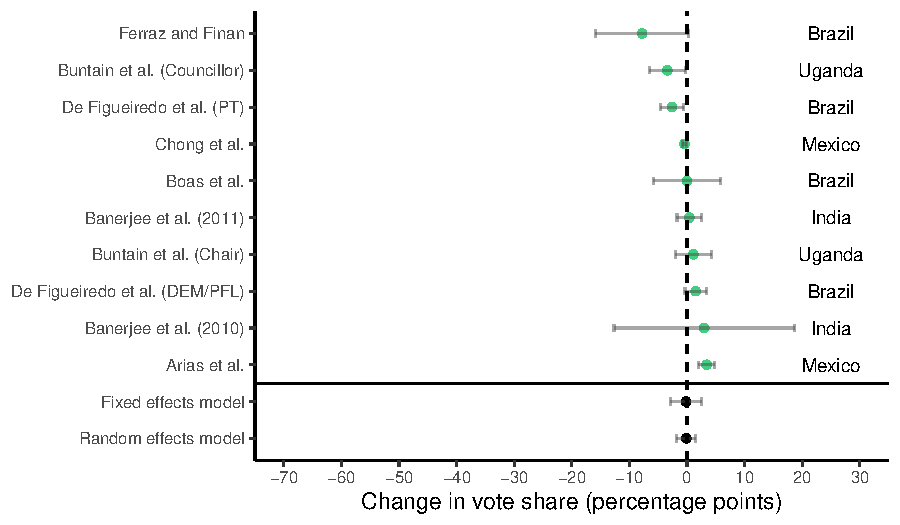
\includegraphics{../figs/field.pdf}
\vspace{0.2cm}
\caption{Field experiments: Average treatment effect of corruption information on incumbent vote share and 95\% confidence intervals}
\small
\vspace{-0.3cm}
\label{fig: meta-field}

\vspace{1.5cm}

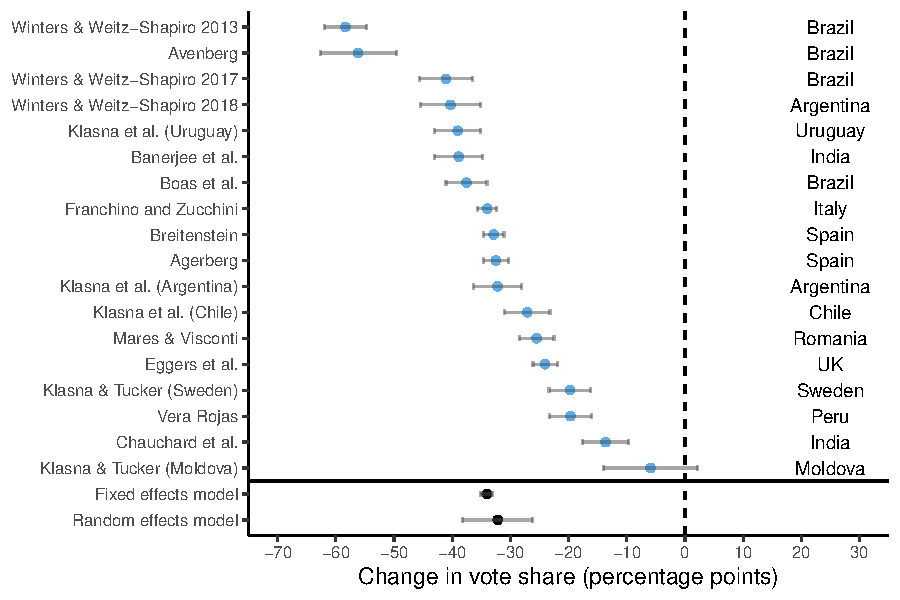
\includegraphics{../figs/survey.pdf}
\vspace{0.2cm}
\caption{Survey experiments: Average treatment effect of corruption information on incumbent vote share and 95\% confidence intervals}
\small
\vspace{-0.3cm}
\label{fig: meta-survey}
\end{figure}

Survey experiments estimate much larger negative treatment effects of providing information about corruption to voters relative to field experiments. In fact, the field-experimental results in \autoref{fig: meta-field} reveal a precisely estimated point estimate of approximately zero and suggest that we cannot reject the null hypothesis of no treatment effect (the 95\% confidence interval is -0.56 to 0.15 percentage points using fixed effects and -2.1 to 1.4 using random effects). By contrast, \autoref{fig: meta-survey} shows that corrupt candidates are punished by respondents by approximately 32 percentage points in survey experiments based on fixed and random effects meta-analysis (the 95\% confidence interval is -32.5 to -31.1 percentage points using fixed effects and -38.2 to 26.2 using random effects). Of the 18 survey experiments, only one shows a null effect \citep{klavsnja2013economy}, while all others are negative and significantly different from zero at conventional levels. 

Examining all studies together, a test for heterogeneity by type of experiment (field or survey) reveals that up to 68\% of the total heterogeneity across studies can be accounted for by a dummy variable for type of experiment (0 = field, 1 = survey) (see \autoref{me_mod}). This dummy variable has a significant association with the effectiveness of the information treatment at the 1\% significance level. In fact, with this dummy variable included, the overall estimate across studies is -0.007, while the point estimate of the survey dummy is -0.315.\footnote{Using a mixed effects model with a survey experiment moderator (see \autoref{me_mod}). With \citet{banerjee2010can} and \citet{banerjee2011informed} excluded from the model, the point estimate of the survey dummy is 0.31 and the heterogeneity accounted for by the survey experiment moderator is 65\% (see \autoref{me_mod_no_banerjee} and \autoref{re_model_no_banerjee}).} This implies that the predicted treatment effect across experiments is not significantly different from zero when an indicator for type of experiment is included in the model. In other words, the majority of the heterogeneity in findings is accounted for by the type of experiment conducted. 

\section{Exploring the discrepancy} \label{sec: discussion}

What accounts for the large difference in treatment effects between field and survey experiments? One possibility is publication bias. Null results may be less likely to be published than significant results, particularly in a survey setting. A second possibility is social desirability bias, which may cause respondents to under-report socially undesirable behavior. Related is hypothetical bias, in which costs are more abstract in hypothetical environments. Survey and field experiments may also not mirror each other and/or real-world voting decisions. Potential ways in which the survey setting may differ from the field are: treatment salience and noncompliance, differences in outcome choices, and costliness/decision complexity. Weak treatments and noncompliance may decrease treatment effect sizes in field experiments. Design decisions may change the choice sets available to respondents. Finally, surveys may not capture the complexity and costliness of real-world voting decisions. It is possible that more complex factorial designs---such as conjoint experiments---may more successfully approximate real-world settings. However, common methods of analysis of conjoint experiments may not capture all theoretical quantities of interest.

\subsection{Publication bias and p-hacking}\label{sec: publication}

Publication bias and p-hacking can lead to overestimated effects in meta-analysis \citep{carter2019correcting, duval2000nonparametric, sterne2001investigating, van2019publication}. While I have identified heterogeneity stemming from the type of experiment performed as a potential source of overestimation, this may reflect that null results are less likely to be published than studies with large and significant negative treatment effects. I therefore now turn to the possibility of publication bias and/or p-hacking. In order to formally test for publication bias, I use the p-curve, examination of funnel plot asymmetry, trim and fill, and the PET-PEESE methods.\footnote{Note the ``best'' technique for assessing bias in meta-analysis varies by circumstance, and the proper test for each circumstance is a subject of active debate. See \citet{carter2019correcting} for a recent overview.}

Of the eight field experimental papers located, only five are published. By contrast, only one of the 15 survey experimental papers remains unpublished, and this is a recent draft. This may reflect that the null results from field experiments are less likely to be published than their survey counterparts with large and highly significant negative treatment effects. While recognizing that the sample size of studies is small, OLS and logistic regression do not indicate that reported p-value is a significant predictor of publication status, although the directionality of coefficients is consistent with lower p-values being more likely to be published (\autoref{p_publication}). However, this simple analysis is complicated by the fact that the p-value associated with the average treatment effect across all subjects may not be the primary p-value of interest in the paper. 

In order to more formally test for publication bias, I first use the p-curve \citep{simonsohn2014p1, simonsohn2014p2, simonsohn2015better}. The p-curve is based on the premise that only ``significant'' results are typically published, and depicts the distribution of statistically significant p-values for a set of published studies. The shape of the p-curve is indicative of whether or not the results of a set of studies are derived from true effects, or from publication bias. If p-values are clustered around 0.05 (i.e. the p-curve is left skewed), this may be evidence of p-hacking, indicating that studies with p-values just below 0.05 are selectively reported. If the p-curve is right skewed and there are more low p-values (0.01), this is evidence of true effects. All significant survey experimental results included in the meta-analysis are significant at the 1\% level, implying that publication bias likely does not explain the large negative treatment effects in survey experiments.\footnote{See \autoref{fig: p_curve_survey} for a visual p-curve for survey experiments and \autoref{p_study} for a list of p-values associated with each study. There is also no indication of publication bias at the 1\% level using this method.} Rather, it is relatively easier to generate large and highly significant negative treatment effects in survey experiments. For field experiments, there is not a large enough number of published experiments to make the p-curve viable.\footnote{See \autoref{fig: p_curve_field} for a visual p-curve for field experiments.} Only six studies are published, and of these only four are significant at at least the 5\% level.

Next, I test for publication bias by examining funnel plot asymmetry. A funnel plot depicts the outcomes from each study on the x-axis and their corresponding standard errors on the y-axis. The chart is overlaid with an inverted triangular confidence interval region (i.e. the funnel), which should contain 95\% of the studies if there is no bias or between study heterogeneity. If studies with insignificant results remain unpublished the funnel plot may be asymmetric. Both visual inspection and regression tests of funnel plot asymmetry reveal an asymmetric funnel plot when survey and field experiments are grouped together (see \autoref{fig: funnel_re_all} and \autoref{tab: funnel}). However, this asymmetry disappears when accounting for heterogeneity by type of experiment, either with the inclusion of a survey experiment moderator (dummy) variable or by analyzing field and survey experiments separately (see \autoref{fig: funnel_all_mod}, \autoref{fig: funnel_re_field}, and \autoref{fig: funnel_re_survey}.). Trim and fill analysis overestimates effect sizes and hypothesizes that three studies are missing from the analysis due to publication bias when analyzing all studies together (see \autoref{fig: funnel_trimfill} and \autoref{trimfill}). However, when trim and fill is used on survey experiments or field experiments as separate subgroups, estimates remain unchanged and no studies are hypothesized to be missing. Similarly, PET-PEESE estimates remain virtually unchanged when survey and field experiments are analyzed as separate subgroups, but exhibit slight overestimation when all experiments are analyzed together.\footnote{See \autoref{petpeese} for the results from PET-PEESE estimation.} \footnote{These results are in accordance with the findings in \citet{terrin2003adjusting}, \citet{peters2007performance}, \citet{carter2019correcting}, and \citet{van2019publication}. \citet{peters2007performance} show that trim and fill returns biased estimates under high between-study heterogeneity. \cite{carter2019correcting} find that both the trim and fill method and p-curve overestimate effect sizes and show high false positive rates in the presence of heterogeneity. \citet{van2016conducting} show similar findings with respect to p-curve estimation, which assumes homogenous effect sizes. PET-PEESE also assumes homogenous effect size and has been shown to be biased when between-study variance in effect sizes is large \citep{van2019publication, stanley2017neither}. \citet{reed2015monte} show that random effects meta-analysis exhibits lower mean-squared error than PET-PEESE under high heterogeneity. \citet{carter2019correcting} recommend standard random effects meta-analysis (as performed here) if publication bias is unlikely.}

In sum, while publication bias cannot be ruled out completely---particularly with such a small sample size of field experiments---there is no smoking gun. This implies that differences in experimental design likely account for the difference in the magnitude of treatment effects in field versus survey experiments, rather than publication bias.


\subsection{Social desirability bias and hypothetical bias}\label{sec: sdb}

A second possible explanation is social desirability or sensitivity bias, in which survey respondents under-report socially undesirable behavior. A respondent may think a particular response will be perceived unfavorably by society as whole, by the researcher(s), or both, and underreport such behavior. In the case of corruption, respondents are likely to perceive corruption as harmful to society, the economy, and their own personal well-being. They may therefore be more likely to choose the socially desirable option (no corruption), particularly when observed by a researcher or afraid of response disclosure.\footnote{Note, however, that social desirability bias differs from norms as norms reflect internalized values, whereas social desirability bias corresponds to misreporting due to fear of judgement by a social referent. Internalized norms would be reflected in both field and survey experimental studies. I would like to thank an anonymous reviewer for this insight. Also see \citet{philp2015realism} for an in-depth discussion of how social norms interact with behavior surrounding corruption.} However, a researcher is not the only social referent to whom a respondent may wish to give a socially desirable response. Respondents also may not wish to admit to themselves that they would vote for a corrupt candidate. Voting against corruption in the abstract may therefore reflect the respondents' actual preferences.

However, sensitivity bias is unlikely to account entirely for the difference in magnitude of treatment effects. A recent meta-analysis finds that sensitivity biases are typically smaller than 10 percentage points, and that respondents underreport vote buying by 8 percentage points on average \citep{blair2018worry}. As vote buying is often considered a form of corruption, the amount of sensitivity bias present in corruption survey experiments may be similar. 

A related but distinct source of bias is hypothetical bias. Hypothetical bias is often found in stated preference surveys in environmental economics, in which respondents report a willingness to pay that is larger than what they will actually pay using their own money as the costs are purely hypothetical \citep{loomis2011s}. For corruption experiments, this would manifest as respondents reporting a willingness to punish corruption larger than in reality as the costs in terms of tradeoffs are purely hypothetical. There are few costs to selecting the socially desirable option in a hypothetical survey experiment. By contrast, the cost of changing one's actual vote (as in field experiments) may be higher. Voters might have pre-existing favorable opinions of real candidates, discount corruption information, or have strong material and/or ideological incentives to stick with their candidate. As the informational treatment will only have an effect on supporters of the corrupt candidate who must change their vote---opponents have already decided not to vote for the candidate---these costs are particularly high. Where anticorruption norms are particularly strong---as in Brazil as highlighted by \citet{boas2018norms}---the magnitude of hypothetical bias may be particularly large. 

How might we overcome social desirability bias and hypothetical bias in survey experiments? For social desirability bias, one option is the use of list experiments. None of the survey experiments included here are list experiments. More complex factorial designs such as conjoint experiments have also been shown to reduce social desirability bias \citep{hainmueller2014causal, horiuchi2018can}. For hypothetical bias, an option is to eschew hypothetical candidates in favor of real candidates. In fact, the only corruption survey experiment to date to use real candidates found a null effect on vote choice \citep{de2011voters}, and \citet{mcdonald2019avoiding} elicits smaller effects in survey experiments using the names of real politicians vs. a hypothetical politician. Of course, for corruption experiments this limits researchers to having actual information regarding the corrupt actions of candidates for ethical reasons.

\subsection{Do field and survey experiments mirror real-world voting decisions?}\label{sec: conjoint}

Even if subjects (voters), treatments (information), and outcome (vote choice) are similar, contextual differences between survey and field experiments may also offer fundamentally different choice sets to voters. These discrepancies between survey and field experimental designs, as well as between the designs of different survey experiments, may alter respondents' potential outcomes and thus capture different estimands. Some possible contextual differences are discussed below. 

\subsubsection{Treatment strength, noncompliance, and declining salience}

Informational treatments may be weaker in field experiments in part because of their method of delivery. Survey treatments tend to be clear and authoritative, and often provide information on the challenger (clean or corrupt).  By contrast, many of the informational treatments utilized in past information and accountability field experiments---e.g. fliers and text messages---provide relatively weak one-time treatments that may even contain information subjects are already aware of. If the goal is to estimate real world effects, interventions should attempt to match those conducted in the real world (e.g. by campaigns, media, etc.). In fact, the natural experiment conducted by \citet{ferraz2008exposing}---which takes advantage of random municipal corruption audits conducted by the Brazilian government---may provide evidence of the effectiveness of stronger treatments. The results of the audits were disseminated naturally by newspapers and political campaigns, and their study provides the largest estimated treatment effect amongst real-world experiments. While not measuring specific vote choice, past experiments using face-to-face canvassing contact have also demonstrated relatively large effects on voter turnout \citep{green2019get, kalla2018minimal}, but these methods have not been used in any information and accountability field experiments to date. 

Treatment effects in field experiments (fliers, newspapers, etc.) may also be weaker in part because they can be missed by segments of the treatment group. More formally, survey experiments do not have noncompliance by design and therefore the average treatment effect (ATE) is equal to the intent-to-treat (ITT) effect,\footnote{It could be argued that survey experiments have noncompliance if a respondent fails to absorb the information in the treatment. However, if there is also noncompliance in survey experiments, the CACE estimates would be even larger than the ITT estimates reported here, and the level of noncompliance in field experiments would need to be correspondingly larger to generate equal treatment effects. I thank an anonymous reviewer for this point.} whereas field experiments present ITT estimates as they are unable to identify which individuals in the treatment area actually received and internalized the informational treatment. Ideally, we would calculate the complier average causal effect (CACE)---the average treatment effect among the subset of respondents who comply with treatment---in field experiments, but we are unfortunately unable to observe compliance in any of the corruption experiments conducted to date.

A theoretical demonstration shows how noncompliance can drastically alter the ITT. The ITT is defined as $ITT = CACE \times \pi_c$ where $\pi_C$ indicates the proportion of compliers in the treatment group. When $\pi_C = 1$, $ITT = CACE = ATE$. If the ITT = -0.0018---as fixed-effects meta-analysis estimates in field experiments---but only 10\% of treated individuals ``complied'' with the treatment by reading the flier sent to them, this implies that the CACE is $\frac{-0.0018}{0.1} = -0.018$, or approximately -2 percentage points. In other words, while the effect of receiving a flier is roughly 0.2 percentage points, the effect of \textit{reading} the flier is -2 percentage points. As the $ITT = CACE \times \pi_c$, any noncompliance necessarily reduces the size of the ITT. However, for the CACE to be equal in both survey and field experiments, the proportion of treatments that would need to remain undelivered in field experiments would have to be over 99\% (i.e. over 99\% of subjects in the treatment group did not receive treatment or were already aware of the corruption information), implying that noncompliance likely does not tell the whole story.

Finally, treatments may be less salient at the time of vote choice in a field setting. Survey treatments are directly presented to respondents who are forced to immediately make a vote choice. \citet{kalla2018minimal} note that this mechanism manifests in campaign contact field experiments, where contact long before election day followed by immediate measurement of outcomes appears to persuade voters, whereas there is a null effect on vote choice on election day. Similarly, \citet{sulitzeanu2019judicial} show that increasing the salience of corruption can increase electoral sanctioning, even without providing any new corruption information. Weaker treatments or lower salience of corruption in field experiments will weaken the treatment effect even amongst compliers (i.e. the CACE), further reducing the ITT. 

Weak treatments, noncompliance, and declining treatment salience over time therefore make it unclear if the zero and null effects observed in field experiments stem from methodological choices or an actual lack of preference updating. Future field experiments should therefore consider using stronger treatments (e.g. canvassing), performing baseline surveys to measure subgroups amongst whom effects may be stronger, utilizing placebo-controlled designs that allow for measurement of noncompliance, and performing repeated measurement of outcome variables over time to capture declining salience.



\subsubsection{Outcome choice}

While vote choice is the outcome variable across all of the experiments investigated here, the choice set offered to voters is not necessarily always identical. Consider a voter's choice between two candidates in a field experiment conducted during an election. A candidate is revealed to be corrupt to voters in a treatment group, but not to voters in control. The treated voter can cast a ballot for corrupt candidate A, or candidate B, who may be clean or corrupt. The control voter can cast a ballot for candidate A or candidate B, and has no corruption information. Now consider a survey experiment with a vignette in which the randomized treatment is whether the corrupt actions of a politician are revealed or not. The treated voter can vote for the corrupt candidate A or not, but no challenger exists. Likewise, the control voter can vote for clean candidate A or not, but no challenger exists. Conjoint experiments overcome this difference, but the option to abstain still does not exist in the survey setting.\footnote{See \citet{eggers2018corruption} and \citet{agerberg2019lesser} for exceptions.} These differences in design offer fundamentally different choice sets to voters, altering respondents' potential outcomes and thus capturing different estimands.

\subsubsection{Complexity, costliness, and conjoint experiments}

Previous researchers have noted that even if voters generally find corruption distasteful, the quality of the information provided or positive candidate attributes and policies may outweigh the negative effects of corruption to voters, mitigating the effects of information provision on vote share.\footnote{See \citet{de2017electoral} for a comprehensive overview.} These mitigating factors will naturally arise in a field setting, but may only be salient to respondents if specifically manipulated in a survey setting. 

A number of survey experiments have therefore added factors other than corruption as mitigating variables, such as information quality, policy, economic benefit, and co-partisanship. Studies have randomized the quality of corruption information\footnote{For example, accusations from an independent anti-corruption authority may be deemed more credible than those from an opposition party, and accusations may be deemed less credible than a conviction.} \citep{botero2015says, breitenstein2019choosing, mares2019voting, banerjee2014poor, weitz2017can, winters2018information}, finding that lower quality information produces smaller negative treatment effects (see \autoref{fig: quality}). Policy stances in line with voter preferences have also been shown to mitigate the impact of corruption \citep{rundquist1977corrupt, franchino2015voting}. Evidence also suggests that respondents are more forgiving of corruption when it benefits them economically \citep{klavsnja2017voters, winters2013lacking}. Evidence of co-partisanship as a limiting factor to corruption deterrence is mixed. \citet{anduiza2013turning}, \citet{agerberg2019lesser}, and \citet{breitenstein2019choosing} show that co-partisanship decreases the importance of corruption to Spanish respondents in survey experiments, and \citet{solaz2018group} find that in-group membership reduces sanction of ``corrupt'' participants in a lab-experiment of UK subjects. However, \citet{klavsnja2017voters} find relatively small effects of co-partisanship in Argentina, Chile, and Uruguay, \citet{rundquist1977corrupt} find null effects in a lab experiment in the US in the 1970s, and \citet{konstantinidis2013sources} find no significant relationship in a survey experiment in Greece. \citet{boas2018norms} posit that abandoning dynastic candidates is particularly costly in Brazil. This evidence suggests that voters punish corruption less when it is costly to do so, and that these costly factors differ by country.  

The fact that moderating variables may dampen the salience of corruption to voters has clearly not been lost on previous researchers. However, in the field setting numerous moderating factors may be salient to the voter. While there is likely no way to capture the complexity of real-world decision making in a survey setting, conjoint experiments allow researchers to randomize many candidate characteristics simultaneously, and thus have become a popular survey method for investigating the relative weights respondents give to different candidate attributes.  In addition, conjoints force respondents to pick between two candidates, better emulating the choice required in an election. Finally, conjoints may minimize social desirability bias as they reduce the probability that the respondent is aware of the researcher's primary experimental manipulation of interest (e.g. corruption).\footnote{This is explicitly mentioned by \citet{hainmueller2014causal}, who argue that conjoint experiments give respondents ``various attributes and thus [they] can often find multiple justifications for a given choice.'' Note, however, that an experiment does not necessarily need to be a conjoint design to have this feature. Conjoint experiments encourage researchers to randomize more attributes and therefore typically contain more complex hypothetical vignettes. However, the same vignette complexity could be achieved without full randomization of these attributes.} 

Researchers often present the results of conjoint experiments as average marginal component effects (AMCEs), then compare the magnitude of these effect sizes. AMCEs represent the unconditional marginal effect of an attribute (e.g. corruption) averaged over all possible values of the other attributes. This measurement is valuable, and crucially allows researchers to test multiple causal hypotheses and compare relative magnitudes of effects between treatments. However, this may or may not be a measure of substantive interest to the researcher, and implies that the AMCE is dependent on the joint distribution of the other attributes in the experiment.\footnote{See \citet{de2019improving} for additional discussion and empirical demonstration of the impact of choice of distribution on the AMCE.} These attributes are usually uniformly randomized. However, in the real world, candidate attributes are not uniformly distributed, so external validity is questionable. When we have a primary treatment of interest, such as corruption, we want to see how a ``typical candidate'' is punished for corruption. However a typical candidate is not a uniformly randomized candidate, but rather a candidate designed to appeal to voters. The corruption AMCE is therefore valid in the context of the experiment---marginalizing over the distribution of all other attributes in the experiment---but would likely be much smaller for a realistic candidate.\footnote{\citet{abramson2019what} also point out that the AMCE represents a weighted average of both intensity and direction. It is therefore important to interpret conjoint results in terms of both intensity and direction of preferences.} This implies that AMCEs have more external validity when the joint distribution of attributes matches the real world and the experiment contains the entire universe of possible attributes.\footnote{The uniform distribution may be reasonable when we are not attempting emulate real-world appearances of attributes---for example to find an optimal policy design from a menu of equally possible options.} 

When researchers have strong theories about the conditions that shape voter decision-making, a more appropriate method may be to calculate average marginal effects in order to present predicted probabilities of voting for a candidate under these conditions.\footnote{This method is utilized by \citet{teele2018ties} to examine the probability of voting for female or male candidates holding other candidate attributes (marital status and number of children) constant, and in corruption experiments by \citet{agerberg2019lesser}, \citet{breitenstein2019choosing}, and \citet{chauchard2019getting}. This method is discussed in more detail by \citet{leeper2019measuring}.} For example, in a conjoint experiment including corruption information, the probability of voting for a candidate that is both corrupt and possesses other particular feature levels (e.g. party membership and/or policy positions), marginalizing across all other features in the experiment.\footnote{Note that standard errors will increase as a result of conditioning on certain combinations of attributes.  However, this can be avoided by utilizing an experimental design that conditions on these features at the design stage.} 

To illustrate this point, I replicate the conjoint experiments conducted in Spain by \citet{breitenstein2019choosing} and in Italy by \citet{franchino2015voting}, and present both AMCEs and predicted probabilities. The \citet{breitenstein2019choosing} re-analysis is presented in the main text, while the re-analysis of \citet{franchino2015voting} is in the appendix.\footnote{Additional predicted probability replications from \citet{mares2019voting} and \citet{chauchard2019getting} can also be found in the appendix.}  Note that I group all corruption accusation levels into a single ``corrupt'' level in my replications. The \citet{breitenstein2019choosing} predicted probabilities are presented as a function of corruption, co-partisanship, political experience, and economic performance. The charts therefore show the probability of preferring a candidate who is always corrupt, but is a co-partisan or not, has low or high experience, and whose district experienced good or bad economic performance, marginalizing across all other features in the experiment. For \citet{franchino2015voting}, the predicted probabilities are presented as a function of corruption and two policy positions---tax policy and same sex marriage---separately for conservative and liberal respondents. The charts therefore show the probability of preferring a candidate who is corrupt, but has particular levels of tax and same sex marriage policy, marginalizing across all other features in the experiment. Note that \citet{franchino2015voting} correctly conclude that their typical ``respondent prefers a corrupt but socially and economically progressive candidate to a clean but conservative one,'' and \citet{breitenstein2019choosing} presents certain predicted probabilities. While I therefore illustrate how predicted probabilities can be used to draw conclusions that may be masked by examination of AMCEs alone, the authors themselves do not make this mistake. I perform the same analysis including only cases where the challenger is clean in the appendix. 

A casual interpretation of the traditional AMCE plots presented in \autoref{fig: b_amce} and \autoref{fig: fz_amce} suggests that it is very unlikely a corrupt candidate would be chosen by a respondent. By contrast, the predicted probabilities plots presented in \autoref{fig: b_margins}, \autoref{fig: fz_margins_right}, and \autoref{fig: fz_margins_left} show that even for corrupt candidates in the conjoint, the right candidate or policy platform presented to the right respondents can garner over 50\% of the predicted hypothetical vote.\footnote{Note that a negative corruption treatment effect is still present. See \autoref{fig: b_margins_corrupt_clean} for a visual depiction of predicted probabilities for both a corrupt and clean candidate. The difference between the point estimates for the corrupt and clean candidate can be interpreted as a  treatment effect. I thank an anonymous reviewer for suggesting this clarification.} Further, the attributes included in these conjoints surely do not represent all candidate attributes relevant to voters, and indeed differ greatly across experiments. As in \cite{agerberg2019lesser}, the level of support for corrupt candidates also varies based on whether or not the challenger is clean (\autoref{fig: b_margins_clean}, \autoref{fig: fz_margins_right_clean}, \autoref{fig: fz_margins_left}). In other words, respondents find it costly to abandon their preferences even if it forces them to select a corrupt candidate, and this costliness varies highly depending on contextual changes and choice of other attributes included in the experiments. 

\begin{figure}[H]
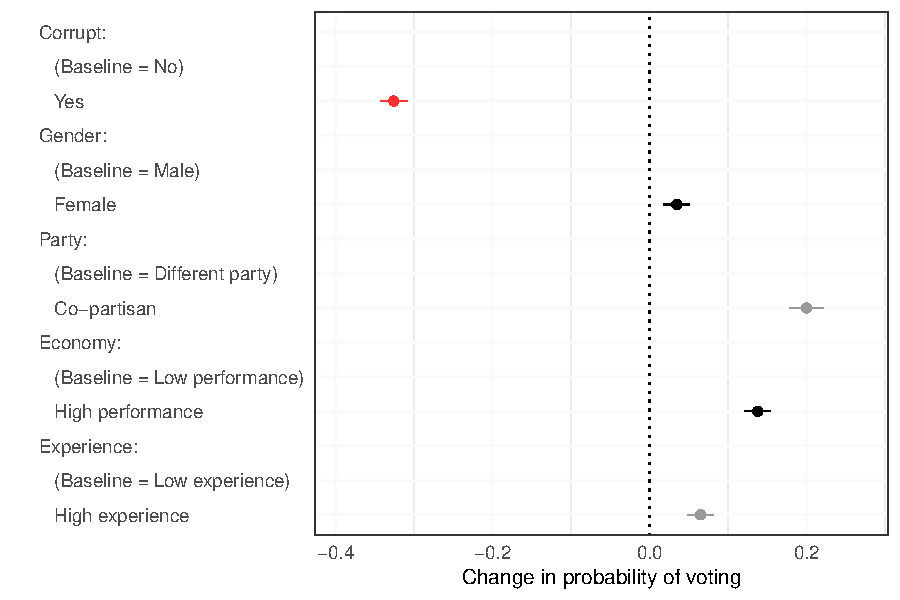
\includegraphics{../figs/b_amce.pdf}
\caption{\citet{breitenstein2019choosing} conjoint: average marginal component effects}
\label{fig: b_amce}
\end{figure}

\begin{figure}[H]
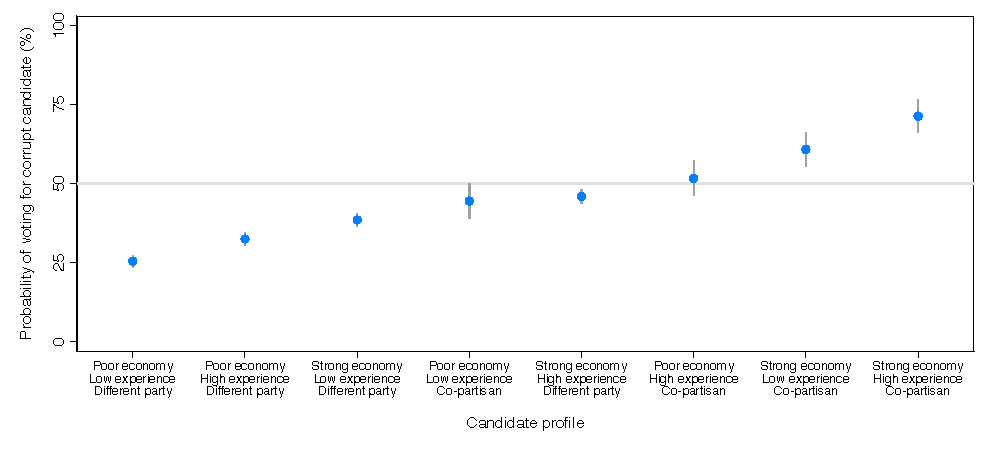
\includegraphics{../figs/b_margins.pdf}
\vspace{0.2cm}
\caption{\citet{breitenstein2019choosing} conjoint: can the right candidate overcome corruption?}
\small
\vspace{-0.3cm}
\label{fig: b_margins}
\end{figure}

Candidate or policy profiles that result in over 50\% of voters selecting a corrupt candidate may not be outliers in real-world scenarios. Unlike in conjoint experiments, real-world candidates' attributes and policy profiles are not selected randomly, but rather represent choices designed to appeal to voters. Voters may also be unsure if the challenger is also corrupt or clean. It may therefore be preferable to analyze conjoint experiments as above, comparing outlier characteristics (e.g. corruption) to realistic candidate profiles that target specific voters, rather than fully randomized candidate profiles.

When the most theoretically relevant tradeoffs are unclear, we may be able to illuminate voter decision making processes through the use of decision trees.\footnote{Decision trees offer a parsimonious way to model fundamental non-linearities in the conjoint data and will typically have lower bias than an OLS-based predicted probability estimator, but may exhibit higher variance.} The decision tree in \autoref{fig: b_tree} was trained using all randomized variables in the \citet{breitenstein2019choosing} conjoint, and the tree was pruned to minimize cross-validated classification error rate.  \autoref{fig: b_tree} draws similar conclusions as the predicted probabilities chart shown in \autoref{fig: b_margins} with respect to what factors matter most to voters. A similar figure depicting corrupt candidates facing clean challengers only can be found in \autoref{fig: b_tree_clean}. 

% Decision trees offer a parsimonious way to model fundamental non-linearities in the conjoint data and likely have lower bias an OLS-based predicted probability estimator, but may exhibit higher variance. 

\begin{figure}[!htb]
\centering
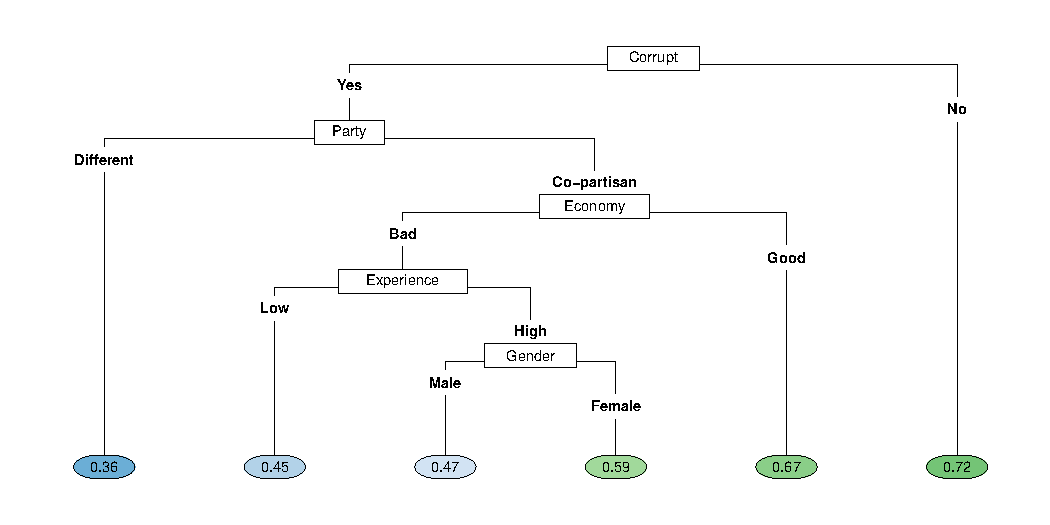
\includegraphics{../figs/b_tree.pdf}
\caption{\citet{breitenstein2019choosing} conjoint decision tree: predicted probabilities of voting for candidate}
\small
\vspace{-0.3cm}
\label{fig: b_tree}
\end{figure}

\section{Discussion}

The field experimental results reported here align with a growing body of literature that shows minimal effects of information provision on voting outcomes. The primary conclusion of the Metaketa I project---which sought to determine if politicians were rewarded for positive information and punished for negative information---was that ``the overall effect of information [provision] across all studies is quite precisely estimated---and not statistically distinguishable from zero'' \citep{dunning2018metaketa}, and a meta-analysis by \citet{kalla2018minimal} suggests that the effect of campaign contact and advertising on voting outcomes in the United States is close to zero in general elections. 

However, we should be careful not to conclude that voters never punish politicians for malfeasance from these experiments, or that field experiments recover truth. Field and natural experiments in other domains have found effects when identifying persuadable voters prior to treatment delivery \citep{rogers2013can, kalla2018minimal}, or when using higher dosage treatments \citep{adidaunder, ferraz2008exposing}.\footnote{While an observational study, \citet{chang2010legislative} also points to the effectiveness of higher dosage treatments.} Combining stronger treatments, measurement of noncompliance, and pre-identification of subgroups most susceptible to persuasion should therefore be a goal of future field experiments. 

Many of the survey experimental studies discuss how their findings may partially stem from the particular conditions of the experiment, claim that they are only attempting to identify tradeoffs or moderating effects, and/or acknowledge the limitations of external validity. However, other studies do not. A common approach is to cite \citet{hainmueller2015validating}, who show similar effects in a vignette, conjoint, and natural experiment. However, \citet{hainmueller2015validating} use closeness in the magnitude of treatment effects between vignettes and the natural experiment as a justification for correspondence between the two methodologies. Their study therefore suggests that the relative importance \textit{and magnitude} of treatment effects should be similar between hypothetical vignettes and the real world, which this meta-analysis shows is not the case with corruption voting. Further, the natural experimental benchmark takes the form of a survey/leaflet sent to voters containing the attributes of immigrants applying for naturalization in Swiss municipalities. The conjoint experiment is therefore able to perfectly mimic the amount of information voters posses in the real world, which is not the case for political candidates.\footnote{\citet{hainmueller2015validating} acknowledge this directly, stating that ``these data provide an ideal behavioral benchmark to evaluate stated preference experiments, because they closely resemble a real-world vignette experiment'' and that ``unlike many other real-world choice situations, in the referendums, the information environment and choice attributes are sufficiently constrained, such that they can be accurately mimicked in a survey experimental design.''} We should therefore be cautious when extrapolating the correspondence between these studies to  cases such as candidate choice experiments.

\section{Conclusion} \label{sec: conclusion}

In an effort to test whether voters adequately hold politicians accountable for malfeasance, researchers have turned to experimental methods to measure the causal effect of learning about politician corruption on vote choice. A meta-analytic assessment of these experiments reveals that conclusions differ drastically depending on whether the experiment was deployed in the field and monitored actual vote choice, versus hypothetical vote choice in a survey setting. Across field experiments, the aggregate treatment effect of providing information about corruption on vote share is approximately zero. By contrast, in survey experiments corrupt candidates are punished by respondents by approximately 32 percentage points. 

I explore publication bias, social desirability bias, and contextual differences in the nature of the experimental designs as possible explanations for the discrepancy between field and survey experimental results. I do not find systematic evidence of publication bias. Social desirability bias may drive some of the difference if survey experiments cause respondents to under-report socially undesirable behavior, and hypothetical bias may cause respondents to not properly internalize the costs of switching their votes.  The survey setting may differ from the field due to contextual differences such as noncompliance, treatment strength, differences in outcome choice sets, and costliness/decision complexity. Noncompliance necessarily decreases treatment effect sizes in field experiments. Weak treatments or lower salience of information to voters on election day versus immediately after treatment receipt will also reduce effect sizes. Previous survey experiments have also shown that treatment effects diminish as the costliness of changing one's vote increases, and these costs are likely to be much higher and more multitudinous in an actual election. The personal cost of changing one's vote may therefore be higher than accepting corruption in many real elections, but not in surveys. 

High-dimension factorial designs such as conjoint experiments may better capture the costly tradeoffs voters make in the survey setting. However, it may be preferable to analyze candidate choice conjoint experiments by comparing the probability of voting for a realistic candidate with outlier characteristics (e.g. corruption) to the probability of voting for the same realistic candidate without this characteristic, rather than examining differences in AMCEs across fully randomized candidate profiles.

These findings suggest that while candidate choice survey experiments may provide information on the directionality of informational treatments in hypothetical scenarios, the point estimates they provide may not be representative of real-world voting behavior. More generally, researchers should exercise caution when interpreting actions taken in hypothetical vignettes as indicative of real world behavior such as voting. However, we should also be careful not to conclude that field experiments always recover generalizable truth due to design decisions and limitations.  


\clearpage
\pagebreak

\pdfbookmark[1]{References}{References}
\bibliography{bibliography}

\pagebreak

\appendix
\setcounter{page}{1}
\setcounter{table}{0}
\setcounter{figure}{0}
\renewcommand\thetable{\Alph{section}.\arabic{table}}
\renewcommand\thefigure{\Alph{section}.\arabic{figure}}
\section{Appendix} \label{Appendix}

\subsection{Lab experiments}

\begin{table}[!htbp] \centering 
  \caption{Lab experiments}
  \label{tab:lab} 
  \small
\begin{tabular}{@{\extracolsep{5pt}} cccccccc} 
\\[-1.8ex]\hline 
\hline \\[-1.8ex] 
 Study & Country & ATE \\ 
 \hline \\[-1.8ex] 
\citet{arvate2017condemning} & Brazil & Negative \\
\citet{azfar2007transparency} & USA & Negative \\
\citet{rundquist1977corrupt}\textsuperscript{1} & USA & Negative \\
\citet{solaz2018group} & UK & Negative \\
\hline \\[-1.8ex] 
\end{tabular} 
 \begin{tablenotes}
\footnotesize
\item \textsuperscript{1} The candidate is always corrupt in the \citet{rundquist1977corrupt} experiment. A ``corruption'' point estimate is therefore not provided in the coefficient plot below.
    \end{tablenotes}
\end{table} 
\FloatBarrier

\vspace{2cm}

\begin{figure}[!htb]
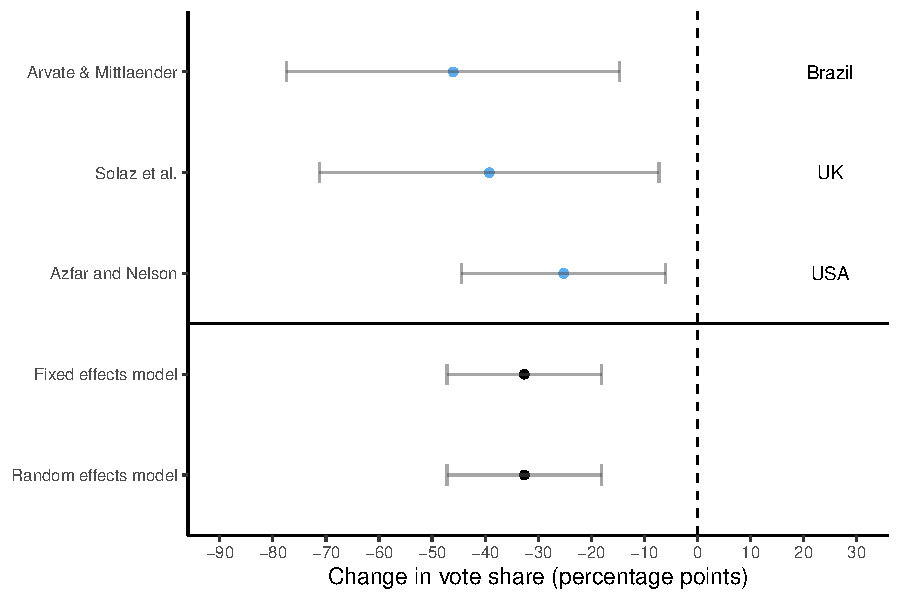
\includegraphics[scale=0.93]{../figs/lab_meta.pdf}
\vspace{0.2cm}
\caption{Lab experiments: Average treatment effect of corruption information on vote share}.
\small
\vspace{-0.3cm}
\label{fig: lab}
\end{figure}

\pagebreak
\subsection{Excluded studies}

\begin{table}[!htbp] \centering 
  \caption{Excluded experiments}
  \label{tab:excluded} 
  \small
\begin{tabular}{@{\extracolsep{0pt}} cccccccc} 
\\[-1.8ex]\hline 
\hline \\[-1.8ex] 
 Study & Type & Reason for exclusion \\ 
\hline \\[-1.8ex] 
\citet{anduiza2013turning} & Survey & Lack of no-corruption control group \\
\citet{botero2015says} & Survey & Lack of no-corruption control group \\
\citet{de2011voters} & Survey & Outcome is hypothetically changing actual vote \\
\citet{green2018publicizing} & Field & Outcome is favorability rating, not vote share \\
\citet{konstantinidis2013sources} & Survey & Lack of no-corruption control group \\
\citet{munoz2012voters} & Survey & Lack of no-corruption control group \\
\citet{rundquist1977corrupt} & Lab & Lack of no-corruption control group \\
\citet{weitz2017can} & Survey & Data identical to \citet{winters2016s} \\
\citet{winters2015political} & Survey & Data identical to \citet{winters2013lacking} \\
\citet{weschle2016punishing} & Survey & Lack of no-corruption control group \\
\hline \\[-1.8ex] 
\end{tabular} 
\end{table} 
\FloatBarrier

\pagebreak

\subsection{Meta-analysis and heterogeneity by type of experiment}


% Table created by stargazer v.5.2.2 by Marek Hlavac, Harvard University. E-mail: hlavac at fas.harvard.edu
% Date and time: Fri, Feb 07, 2020 - 09:49:14
\begin{table}[!htbp] \centering 
  \caption{Meta-analysis by type of experiment} 
  \label{meta_type} 
\begin{tabular}{@{\extracolsep{30pt}} ccc} 
\\[-1.8ex]\hline 
\hline \\[-1.8ex] 
Value & Estimate & 95\% CI \\ 
\hline \\[-1.8ex] 
Field: weighted fixed effects  & -0.002 & -0.006 to 0.001 \\ 
 & (0.002) &  \\ 
Field: random effects & -0.003 & -0.021 to 0.014 \\ 
 & (0.009) &  \\ 
Survey: weighted fixed effects  & -0.319 & -0.326 to -0.312 \\ 
 & (0.004) &  \\ 
Survey: random effects & -0.322 & -0.382 to -0.262 \\ 
 & (0.031) &  \\ 
\hline \\[-1.8ex] 
\multicolumn{3}{l}{\parbox[t]{\textwidth}{\footnotesize \textit{Note:} Standard errors in parenthesis. Figures rounded to nearest thousandth decimal place.}} \\ 
\end{tabular} 
\end{table} 


\vspace*{-0.5cm}


% Table created by stargazer v.5.2.2 by Marek Hlavac, Harvard University. E-mail: hlavac at fas.harvard.edu
% Date and time: Tue, Oct 22, 2019 - 16:18:07
\begin{table}[!htbp] \centering 
  \caption{Random effects meta-analysis (all studies)} 
  \label{re_model} 
\begin{tabular}{@{\extracolsep{5pt}} cc} 
\\[-1.8ex]\hline 
\hline \\[-1.8ex] 
Value & Estimate \\ 
\hline \\[-1.8ex] 
Estimate & -0.214 \\ 
 & (0.036) \\ 
Estimated total heterogeneity & 0.036 \\ 
 & (0.01) \\ 
\hline \\[-1.8ex] 
\multicolumn{2}{l}{\parbox[t]{\textwidth}{\footnotesize \textit{Note:} Standard errors in parenthesis. Figures rounded to nearest thousandth decimal place.}} \\ 
\end{tabular} 
\end{table} 


\vspace*{-0.5cm}


% Table created by stargazer v.5.2.2 by Marek Hlavac, Harvard University. E-mail: hlavac at fas.harvard.edu
% Date and time: Wed, Jan 29, 2020 - 17:55:53
\begin{table}[!htbp] \centering 
  \caption{Mixed effects meta-analysis with survey experiment moderator} 
  \label{me_mod} 
\begin{tabular}{@{\extracolsep{5pt}} ccc} 
\\[-1.8ex]\hline 
\hline \\[-1.8ex] 
Value & Estimate & 95\% CI \\ 
\hline \\[-1.8ex] 
Constant & -0.007 & -0.074 to 0.06 \\ 
 & (0.034) &  \\ 
Survey experiment moderator & -0.315 & -0.398 to -0.231 \\ 
 & (0.043) &  \\ 
Residual heterogenity with moderator & 0.011 & 0.005 to 0.017 \\ 
 & (0.003) &  \\ 
Heterogenity accounted for & 67.97\% &  \\ 
 &  &  \\ 
\hline \\[-1.8ex] 
\multicolumn{3}{l}{\parbox[t]{\textwidth}{\footnotesize \textit{Note:} Standard errors in parenthesis. Figures rounded to nearest thousandth decimal place.}} \\ 
\end{tabular} 
\end{table} 


\vspace{0.75cm}

\noindent
``Heterogeneity accounted for'' is calculated as: $\dfrac{(\text{Total heterogeneity} - \text{Residual heterogeneity})}{(\text{Total heterogeneity})}$

\pagebreak


\pagebreak
\subsection{Robustness checks}

\vspace{-0.5cm}
\begin{figure}[!htb]
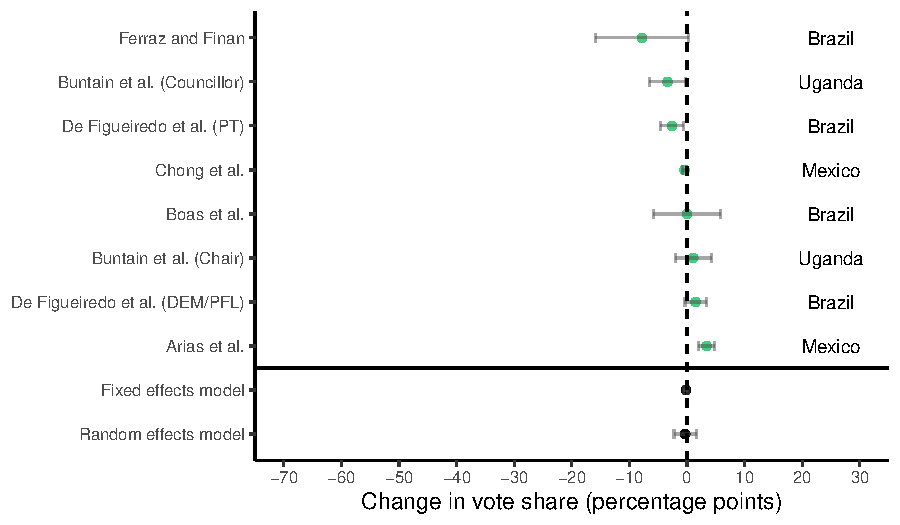
\includegraphics[scale=0.93]{../figs/field_no_banerjee.pdf}
\vspace{0.2cm}
\caption{Field experiments: Average treatment effect of corruption information on incumbent vote share (excluding \cite{banerjee2010can} and \citet{banerjee2011informed})}.
\small
\vspace{-0.3cm}
\label{fig: meta-field_no_banerjee}

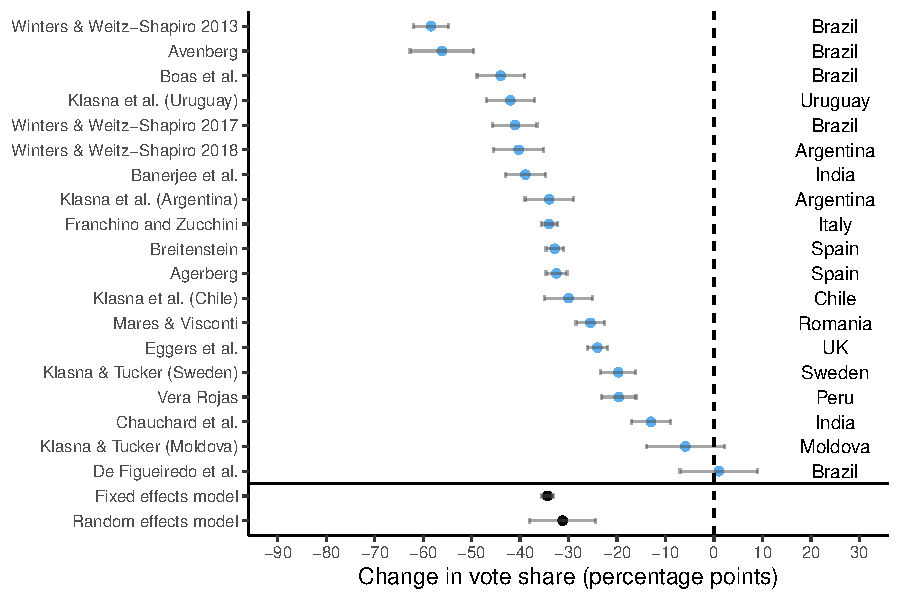
\includegraphics[scale=0.93]{../figs/survey_defig.pdf}
\vspace{0.2cm}
\caption{Survey experiments: Average treatment effect of corruption information on incumbent vote share (including \cite{de2011voters})}.
\small
\vspace{-0.3cm}
\label{fig: meta-field_defig}
\end{figure}

\pagebreak


% Table created by stargazer v.5.2.2 by Marek Hlavac, Harvard University. E-mail: hlavac at fas.harvard.edu
% Date and time: Thu, Feb 06, 2020 - 17:51:54
\begin{table}[!htbp] \centering 
  \caption{Meta-analysis (all field experiments excluding \citet{banerjee2010can} and \citet{banerjee2011informed})} 
  \label{meta_no_banerjee} 
\begin{tabular}{@{\extracolsep{30pt}} ccc} 
\\[-1.8ex]\hline 
\hline \\[-1.8ex] 
Value & Estimate & 95\% CI \\ 
\hline \\[-1.8ex] 
Field: weighted fixed effects  & -0.002 & -0.006 to 0.002 \\ 
 & (0.002) &  \\ 
Field: random effects & -0.003 & -0.022 to 0.016 \\ 
 & (0.01) &  \\ 
\hline \\[-1.8ex] 
\multicolumn{3}{l}{\parbox[t]{\textwidth}{\footnotesize \textit{Note:} Standard errors in parenthesis. Figures rounded to nearest thousandth decimal place.}} \\ 
\end{tabular} 
\end{table} 



% Table created by stargazer v.5.2.2 by Marek Hlavac, Harvard University. E-mail: hlavac at fas.harvard.edu
% Date and time: Fri, Oct 25, 2019 - 14:19:59
\begin{table}[!htbp] \centering 
  \caption{Random effects meta-analysis (all studies excluding \citet{banerjee2010can} and \citet{banerjee2011informed})} 
  \label{re_model_no_banerjee} 
\begin{tabular}{@{\extracolsep{5pt}} cc} 
\\[-1.8ex]\hline 
\hline \\[-1.8ex] 
Value & Estimate \\ 
\hline \\[-1.8ex] 
Estimate & -0.231 \\ 
 & (0.037) \\ 
Estimated total heterogeneity & 0.035 \\ 
 & (0.01) \\ 
\hline \\[-1.8ex] 
\multicolumn{2}{l}{\parbox[t]{\textwidth}{\footnotesize \textit{Note:} Standard errors in parenthesis. Figures rounded to nearest thousandth decimal place.}} \\ 
\end{tabular} 
\end{table} 



% Table created by stargazer v.5.2.2 by Marek Hlavac, Harvard University. E-mail: hlavac at fas.harvard.edu
% Date and time: Fri, Nov 08, 2019 - 14:52:34
\begin{table}[!htbp] \centering 
  \caption{Mixed effects meta-analysis with survey experiment moderator (excluding \citet{banerjee2010can} and \citet{banerjee2011informed})} 
  \label{me_mod_no_banerjee} 
\begin{tabular}{@{\extracolsep{5pt}} cc} 
\\[-1.8ex]\hline 
\hline \\[-1.8ex] 
Value & Estimate \\ 
\hline \\[-1.8ex] 
Constant & -0.009 \\ 
 & (0.039) \\ 
Survey experiment moderator & -0.313 \\ 
 & (0.047) \\ 
Residual heterogenity with moderator & 0.012 \\ 
 & (0.004) \\ 
Heterogenity accounted for & 64.699\% \\ 
 &  \\ 
\hline \\[-1.8ex] 
\multicolumn{2}{l}{\parbox[t]{\textwidth}{\footnotesize \textit{Note:} Standard errors in parenthesis. Figures rounded to nearest thousandth decimal place.}} \\ 
\end{tabular} 
\end{table} 



% Table created by stargazer v.5.2.2 by Marek Hlavac, Harvard University. E-mail: hlavac at fas.harvard.edu
% Date and time: Mon, Jan 27, 2020 - 22:33:04
\begin{table}[!htbp] \centering 
  \caption{Meta-analysis (all survey experiments including \citet{de2011voters}} 
  \label{meta_survey_defig} 
\begin{tabular}{@{\extracolsep{30pt}} ccc} 
\\[-1.8ex]\hline 
\hline \\[-1.8ex] 
Value & Estimate & 95\% CI \\ 
\hline \\[-1.8ex] 
Survey: weighted fixed effects  & -0.315 & -0.322 to -0.308 \\ 
 & (0.004) &  \\ 
Survey: random effects & -0.305 & -0.371 to -0.239 \\ 
 & (0.034) &  \\ 
\hline \\[-1.8ex] 
\multicolumn{3}{l}{\parbox[t]{\textwidth}{\footnotesize \textit{Note:} Standard errors in parenthesis. Figures rounded to nearest thousandth decimal place.}} \\ 
\end{tabular} 
\end{table} 



\clearpage
\pagebreak

\subsection{Publication bias}


% Table created by stargazer v.5.2.2 by Marek Hlavac, Harvard University. E-mail: hlavac at fas.harvard.edu
% Date and time: Thu, Jan 23, 2020 - 15:00:07
\begin{table}[!htbp] \centering 
  \caption{P-values by study} 
  \label{p_study} 
\begin{tabular}{@{\extracolsep{5pt}} cccc} 
\\[-1.8ex]\hline 
\hline \\[-1.8ex] 
Study & Experiment Type & Average Treatment Effect & P value \\ 
\hline \\[-1.8ex] 
Winters and Weitz-Shapiro 2013 & Survey & -58.36 & \textless 0.01 \\ 
Avenberg & Survey & -56.17 & \textless 0.01 \\ 
Winters and Weitz-Shapiro 2017 & Survey & -41.08 & \textless 0.01 \\ 
Winters and Weitz-Shapiro 2018 & Survey & -40.29 & \textless 0.01 \\ 
Klasna et al. (Uruguay) & Survey & -39.05 & \textless 0.01 \\ 
Banerjee et al. & Survey & -38.9 & \textless 0.01 \\ 
Boas et al. & Survey & -37.55 & \textless 0.01 \\ 
Franchino and Zucchini & Survey & -33.99 & \textless 0.01 \\ 
Breitenstein & Survey & -32.87 & \textless 0.01 \\ 
Agerberg & Survey & -32.5 & \textless 0.01 \\ 
Klasna et al. (Argentina) & Survey & -32.21 & \textless 0.01 \\ 
Klasna et al. (Chile) & Survey & -27.12 & \textless 0.01 \\ 
Mares and Visconti & Survey & -25.5 & \textless 0.01 \\ 
Eggers et al. & Survey & -24.04 & \textless 0.01 \\ 
Klasna and Tucker (Sweden) & Survey & -19.77 & \textless 0.01 \\ 
Vera Rojas & Survey & -19.67 & \textless 0.01 \\ 
Chauchard et al. & Survey & -13.66 & \textless 0.01 \\ 
Klasna and Tucker (Moldova) & Survey & -5.9 & \textless 0.01 \\ 
Arias et al. & Field & 3.4 & \textless 0.01 \\ 
Buntain et al. (Councillor) & Field & -3.4 & \textless 0.05 \\ 
De Figueiredo et al. (PT) & Field & -2.6 & \textless 0.05 \\ 
Chong et al. & Field & -0.43 & \textless 0.05 \\ 
Ferraz and Finan & Natural & -7.8 & \textless 0.1 \\ 
Banerjee et al. (2011) & Field & -1.5 & \textgreater 0.1 \\ 
Boas et al. & Field & 0 & \textgreater 0.1 \\ 
Buntain et al. (Chair) & Field & 1.1 & \textgreater 0.1 \\ 
De Figueiredo et al. (DEM/PFL) & Field & 1.5 & \textgreater 0.1 \\ 
Banerjee et al. (2010) & Field & 3 & \textgreater 0.1 \\ 
\hline \\[-1.8ex] 
\end{tabular} 
\end{table} 

\noindent
\footnotesize
Notes: Publication status as of November 2019. All p-values rounded to the nearest thousandth decimal place.  Reported p-value is the p-value associated with the corruption ATE directly reported in the paper if available. If not available, p-values are  reconstructed from point estimates, standard errors, and sample size in regression tables. Replicated p-values are shown for all studies which were fully replicated. 


% Table created by stargazer v.5.2.2 by Marek Hlavac, Harvard University. E-mail: hlavac at fas.harvard.edu
% Date and time: Wed, Jun 26, 2019 - 15:53:40
% Requires LaTeX packages: dcolumn 
\begin{table}[!htbp] \centering 
  \caption{Do p-values predict publication status?} 
  \label{p_publication} 
\begin{tabular}{@{\extracolsep{5pt}}lD{.}{.}{-2} D{.}{.}{-2} } 
\\[-1.8ex]\hline 
\hline \\[-1.8ex] 
 & \multicolumn{2}{c}{\textit{Dependent variable:}} \\ 
\cline{2-3} 
\\[-1.8ex] & \multicolumn{2}{c}{Published} \\ 
 & \multicolumn{1}{c}{OLS} & \multicolumn{1}{c}{Logit} \\ 
\hline \\[-1.8ex] 
 Reference: P less than 0.01 & 0.89^{***} & 2.08^{***} \\ 
  & (0.10) & (0.75) \\ 
  P less than 0.05 & -0.39 & -2.08^{*} \\ 
  & (0.23) & (1.25) \\ 
  P less than 0.1 & 0.11 & 14.49 \\ 
  & (0.42) & (2,399.54) \\ 
  P greater than 0.1 & -0.39^{*} & -2.08^{*} \\ 
  & (0.19) & (1.11) \\ 
 \hline \\[-1.8ex] 
Observations & \multicolumn{1}{c}{29} & \multicolumn{1}{c}{29} \\ 
\hline 
\hline \\[-1.8ex] 
\textit{Note:}  & \multicolumn{2}{r}{$^{*}$p$<$0.1; $^{**}$p$<$0.05; $^{***}$p$<$0.01} \\ 
\end{tabular} 
\end{table} 



% Table created by stargazer v.5.2.2 by Marek Hlavac, Harvard University. E-mail: hlavac at fas.harvard.edu
% Date and time: Wed, Jan 29, 2020 - 18:58:47
\begin{table}[!htbp] \centering 
  \caption{Regression tests for funnel plot asymmetry} 
  \label{tab: funnel} 
\begin{tabular}{@{\extracolsep{5cm}} cc} 
\\[-1.8ex]\hline 
\hline \\[-1.8ex] 
Studies included & p value \\ 
\hline \\[-1.8ex] 
All & $0.0003$ \\ 
All with moderator & $0.896$ \\ 
Field & $0.954$ \\ 
Survey & $0.821$ \\ 
\hline \\[-1.8ex] 
\end{tabular} 
\end{table} 



% Table created by stargazer v.5.2.2 by Marek Hlavac, Harvard University. E-mail: hlavac at fas.harvard.edu
% Date and time: Wed, Feb 05, 2020 - 18:25:07
\begin{table}[!htbp] \centering 
  \caption{Trim and fill estimates by subgroup} 
  \label{trimfill} 
\begin{tabular}{@{\extracolsep{30pt}} ccc} 
\\[-1.8ex]\hline 
\hline \\[-1.8ex] 
Value & Estimate & 95\% CI \\ 
\hline \\[-1.8ex] 
All experiments: random effects  & -0.237 & -0.307 to -0.168 \\ 
 & (0.035) &  \\ 
Field: random effects & -0.003 & -0.021 to 0.014 \\ 
 & (0.009) &  \\ 
Survey: random effects & -0.322 & -0.382 to -0.262 \\ 
 & (0.031) &  \\ 
\hline \\[-1.8ex] 
\multicolumn{3}{l}{\parbox[t]{\textwidth}{\footnotesize \textit{Note:} Standard errors in parenthesis. Figures rounded to nearest thousandth decimal place.}} \\ 
\end{tabular} 
\end{table} 



% Table created by stargazer v.5.2.2 by Marek Hlavac, Harvard University. E-mail: hlavac at fas.harvard.edu
% Date and time: Tue, Feb 04, 2020 - 19:07:13
\begin{table}[!htbp] \centering 
  \caption{PET-PEESE estimates by subgroup} 
  \label{petpeese} 
\begin{tabular}{@{\extracolsep{30pt}} ccc} 
\\[-1.8ex]\hline 
\hline \\[-1.8ex] 
Value & Estimate & 95\% CI \\ 
\hline \\[-1.8ex] 
All experiments & -0.048 & -0.099 to 0.002 \\ 
 & (0.026) &  \\ 
Field experiments & -0.002 & -0.013 to 0.009 \\ 
 & (0.006) &  \\ 
Survey experiments & -0.313 & -0.377 to -0.25 \\ 
 & (0.032) &  \\ 
\hline \\[-1.8ex] 
\multicolumn{3}{l}{\parbox[t]{\textwidth}{\footnotesize \textit{Note:} Standard errors in parenthesis. Figures rounded to nearest thousandth decimal place.}} \\ 
\end{tabular} 
\end{table} 


\clearpage

\begin{figure}[!htb]
\begin{centering}
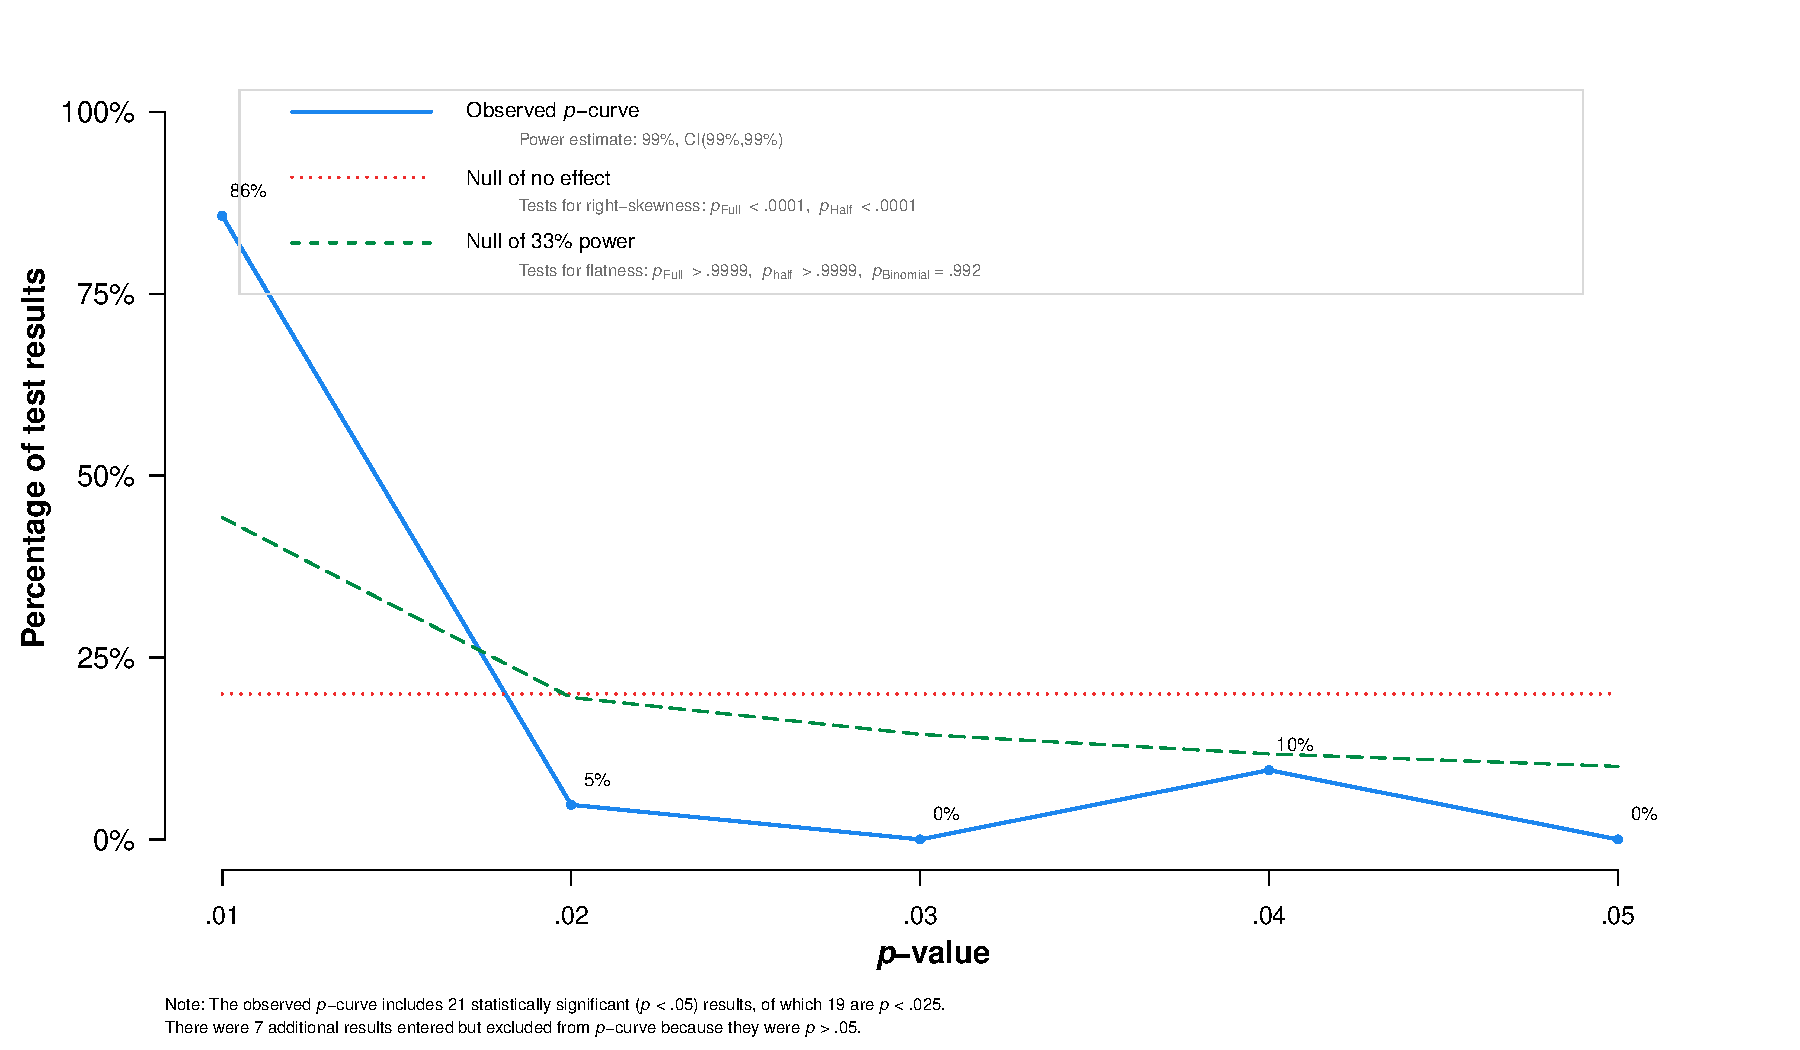
\includegraphics[scale=0.55]{../figs/p_curve_all.pdf}
\vspace{0.1cm}
\caption{P-curve: all experiments}.
\small
\vspace{-0.8cm}
\label{fig: p_curve_all}
\end{centering}
\end{figure}

\begin{figure}[!htb]
\begin{centering}
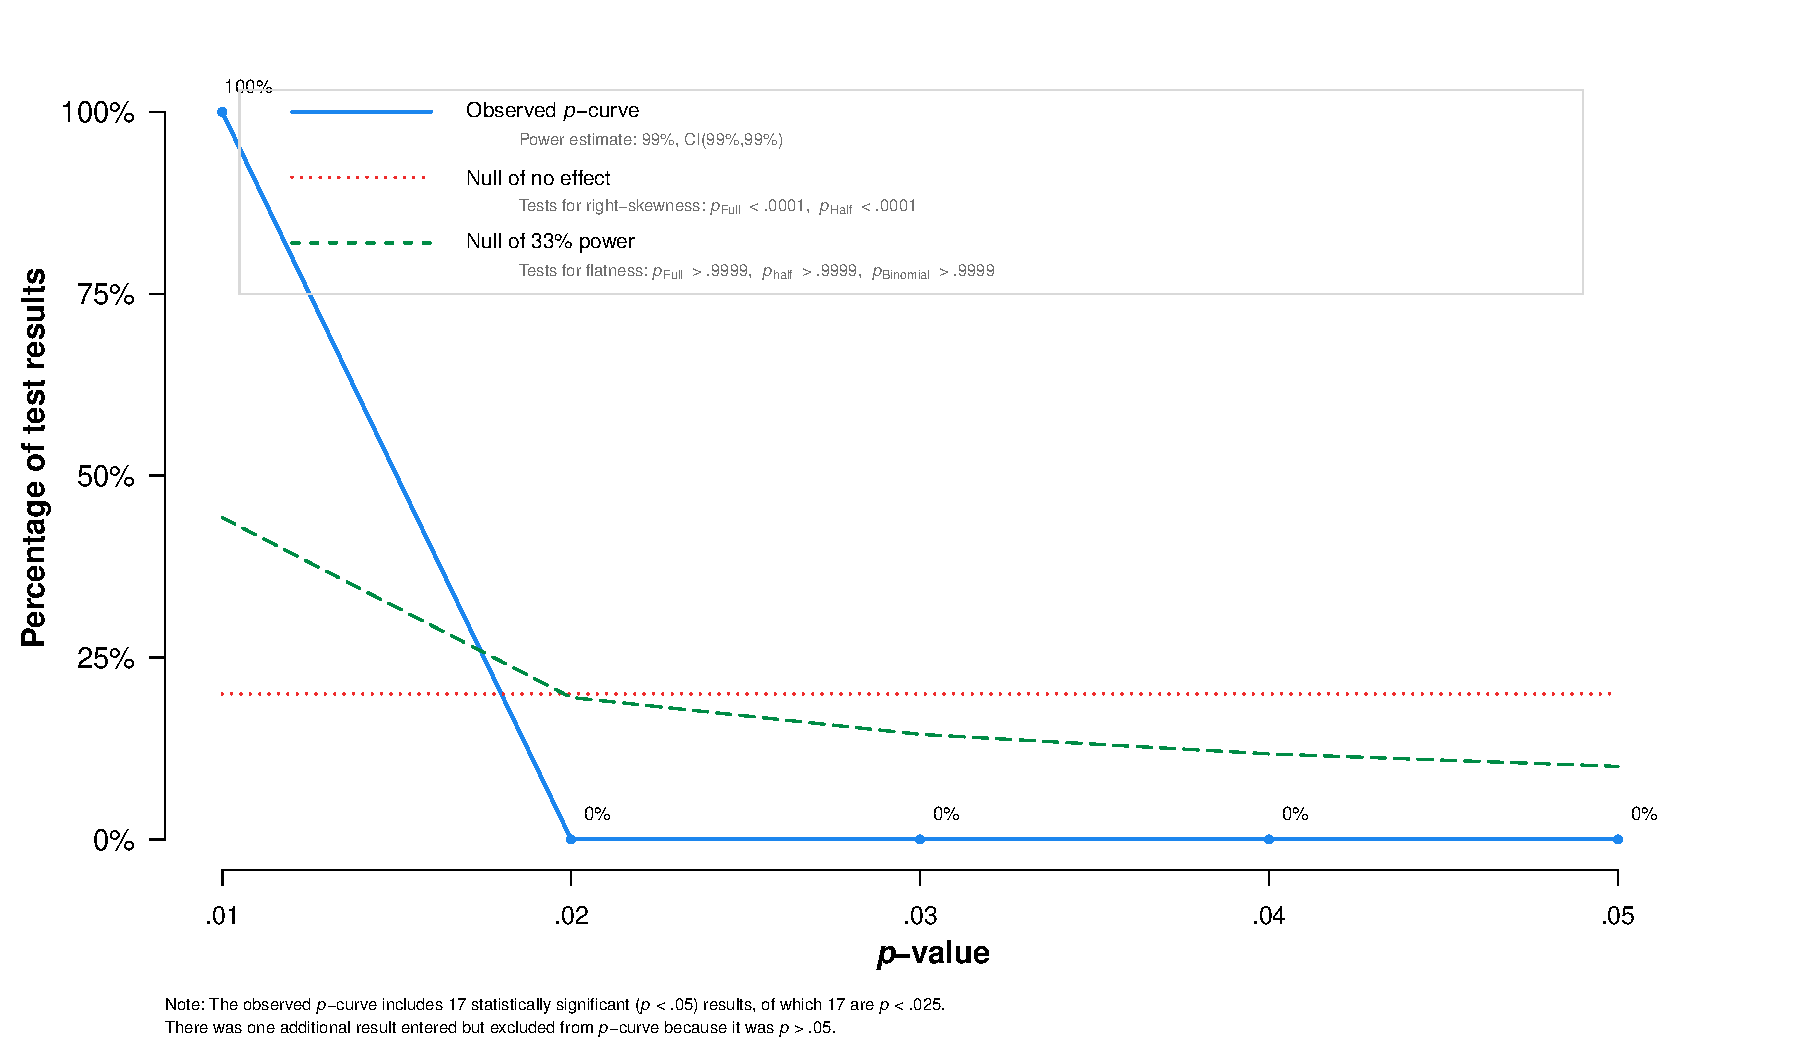
\includegraphics[scale=0.55]{../figs/p_curve_survey.pdf}
\vspace{0.1cm}
\caption{P-curve: survey experiments}.
\small
\vspace{-0.8cm}
\label{fig: p_curve_survey}
\end{centering}
\end{figure}

\clearpage

\begin{figure}[!htb]
\begin{centering}
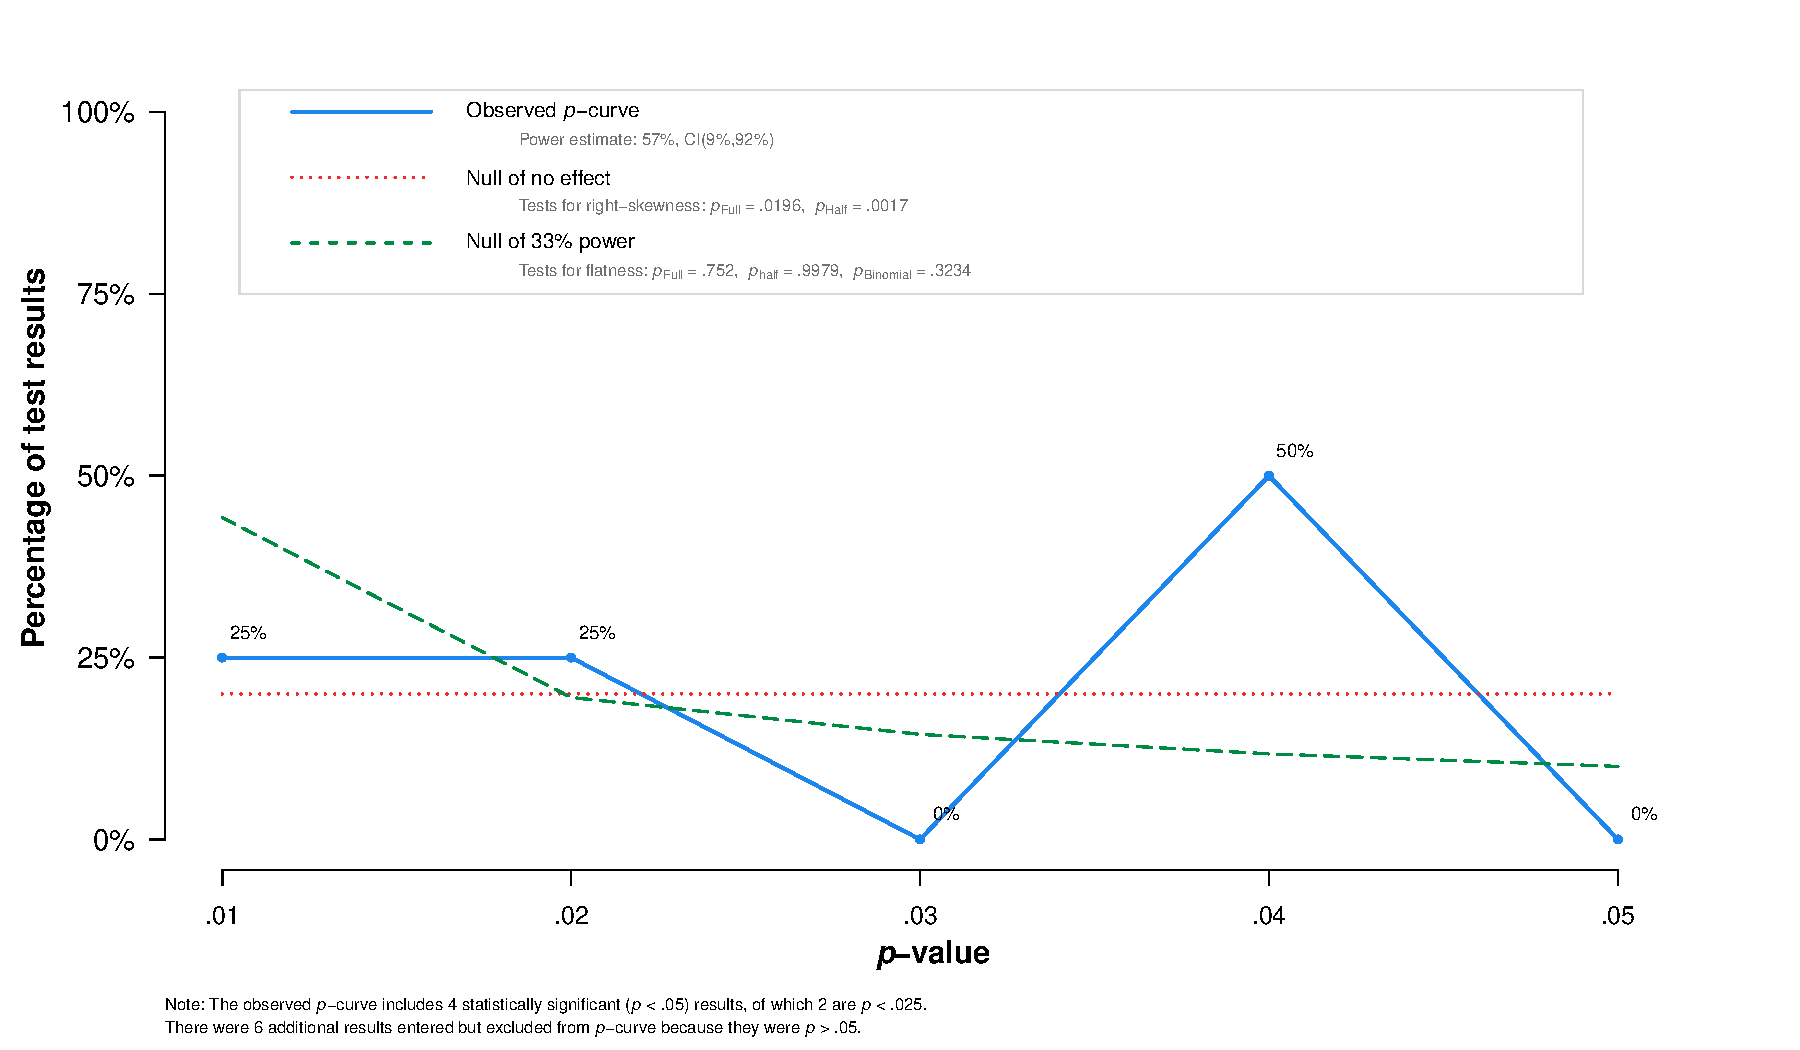
\includegraphics[scale=0.55]{../figs/p_curve_field.pdf}
\vspace{0.1cm}
\caption{P-curve: field experiments}.
\small
\vspace{-0.8cm}
\label{fig: p_curve_field}
\end{centering}
\end{figure}

\clearpage

\begin{figure}[!htb]
\begin{centering}
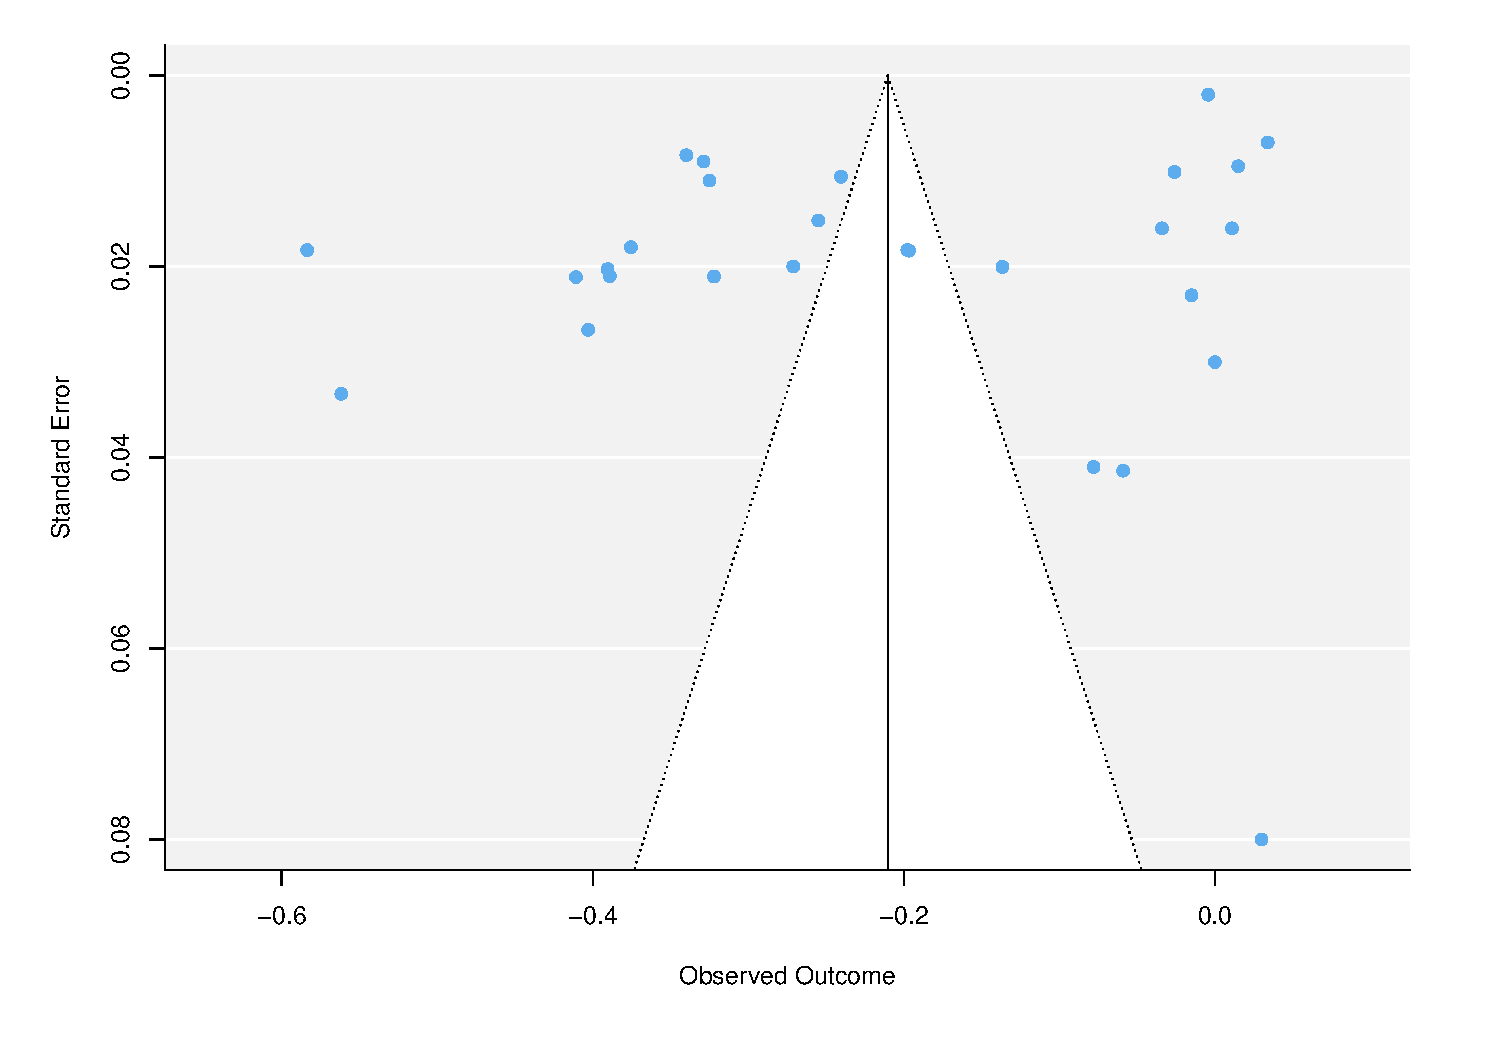
\includegraphics[scale=0.55]{../figs/funnel_re_all.pdf}
\vspace{0.1cm}
\caption{Funnel plot: all experiments}.
\small
\vspace{-0.8cm}
\label{fig: funnel_re_all}
\end{centering}
\end{figure}

\begin{figure}[!htb]
\begin{centering}
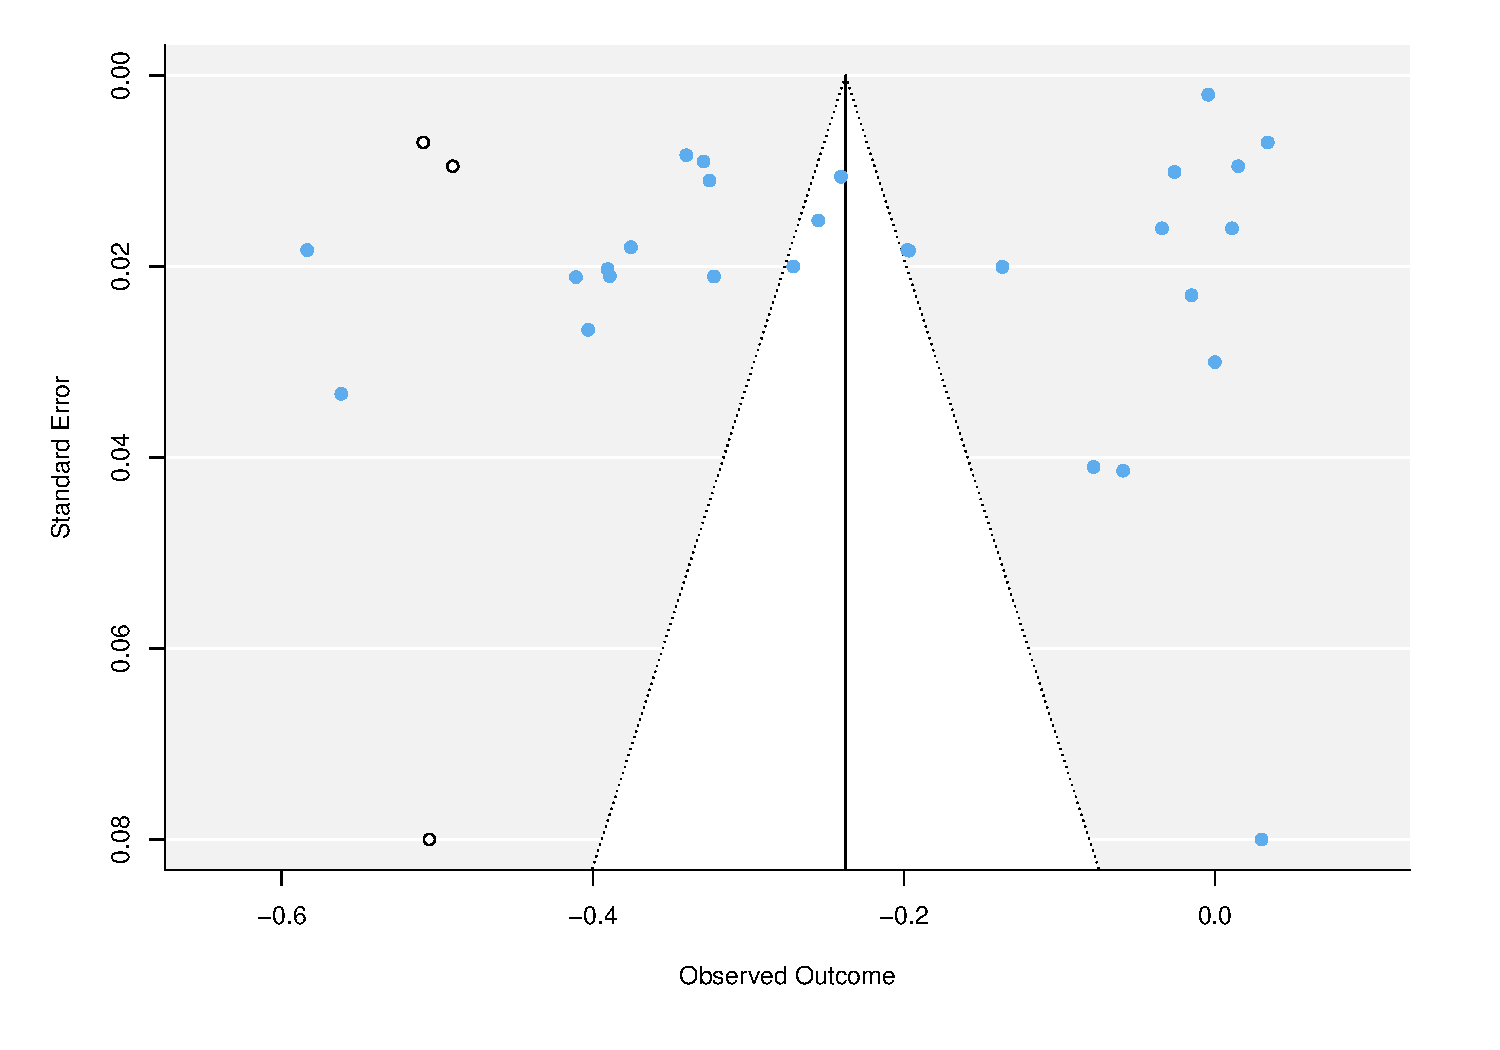
\includegraphics[scale=0.55]{../figs/funnel_trimfill.pdf}
\vspace{0.2cm}
\caption{Funnel plot including trim and fill ``missing'' studies: all experiments}.
\small
\vspace{-0.6cm}
Note: Actual studies in blue and estimated missing studies in white.
\label{fig: funnel_trimfill}
\end{centering}
\end{figure}

\vspace{1cm}

\begin{figure}[!htb]
\begin{centering}
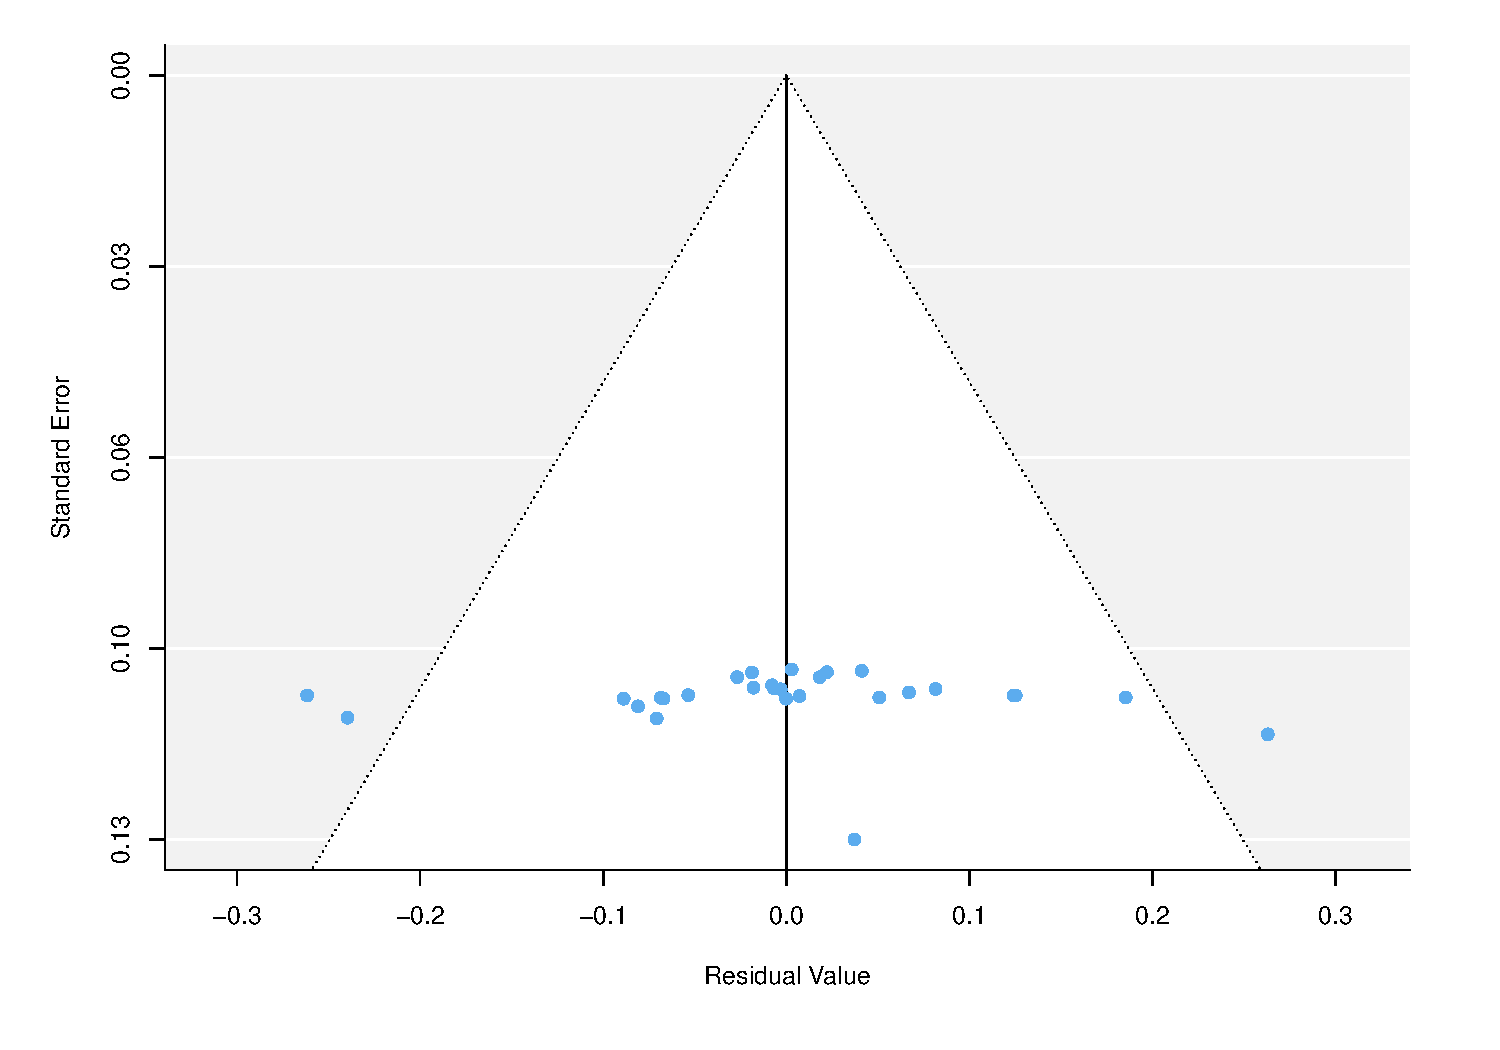
\includegraphics[scale=0.55]{../figs/funnel_all_mod.pdf}
\vspace{0.2cm}
\caption{Funnel plot: all experiments with field experiment moderator}.
\small
\vspace{-0.25cm}
\label{fig: funnel_all_mod}
\end{centering}
\end{figure}

\begin{figure}[!htb]
\begin{centering}
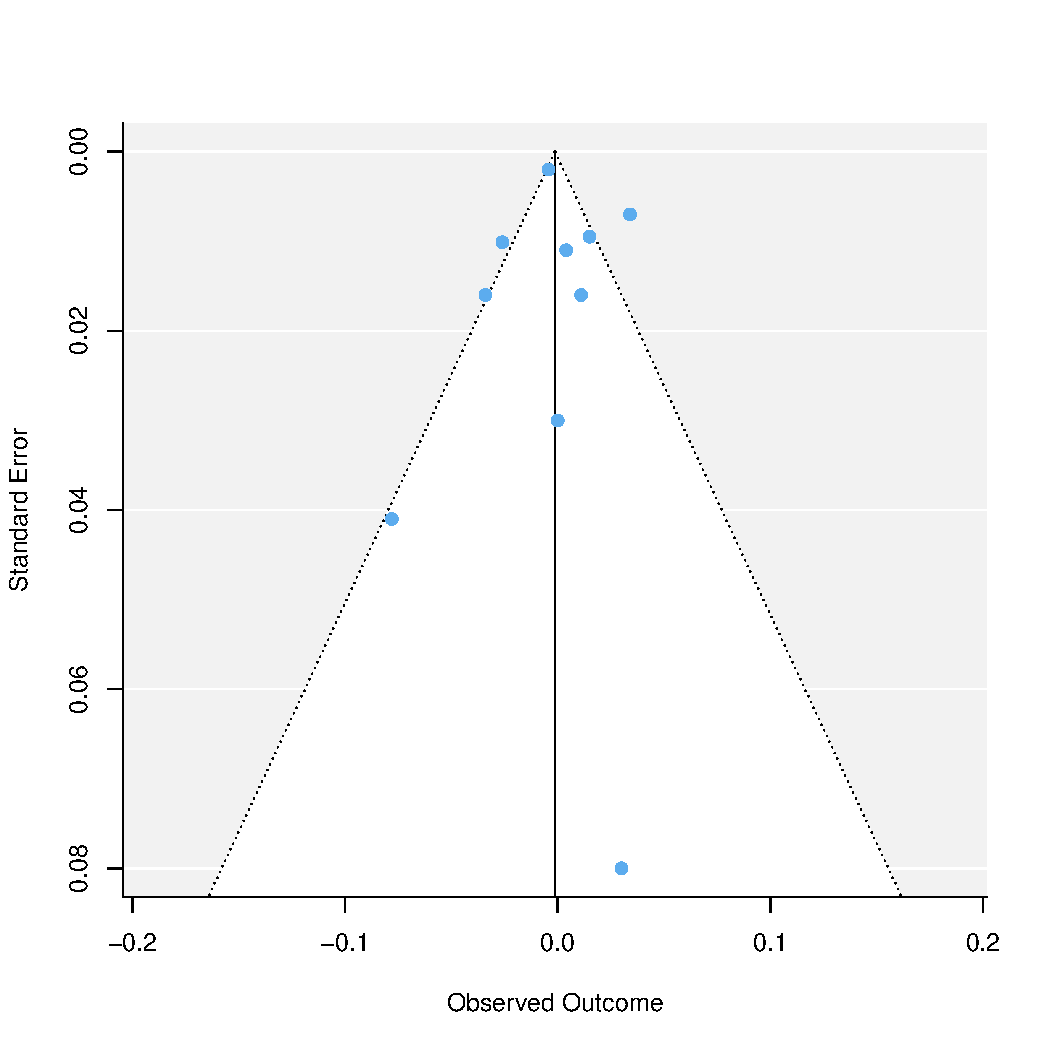
\includegraphics[scale=0.57]{../figs/funnel_re_field.pdf}
\vspace{0.2cm}
\caption{Funnel plot: field experiments}.
\small
\vspace{-0.3cm}
\label{fig: funnel_re_field}
\end{centering}
\end{figure}

\begin{figure}[!htb]
\begin{centering}
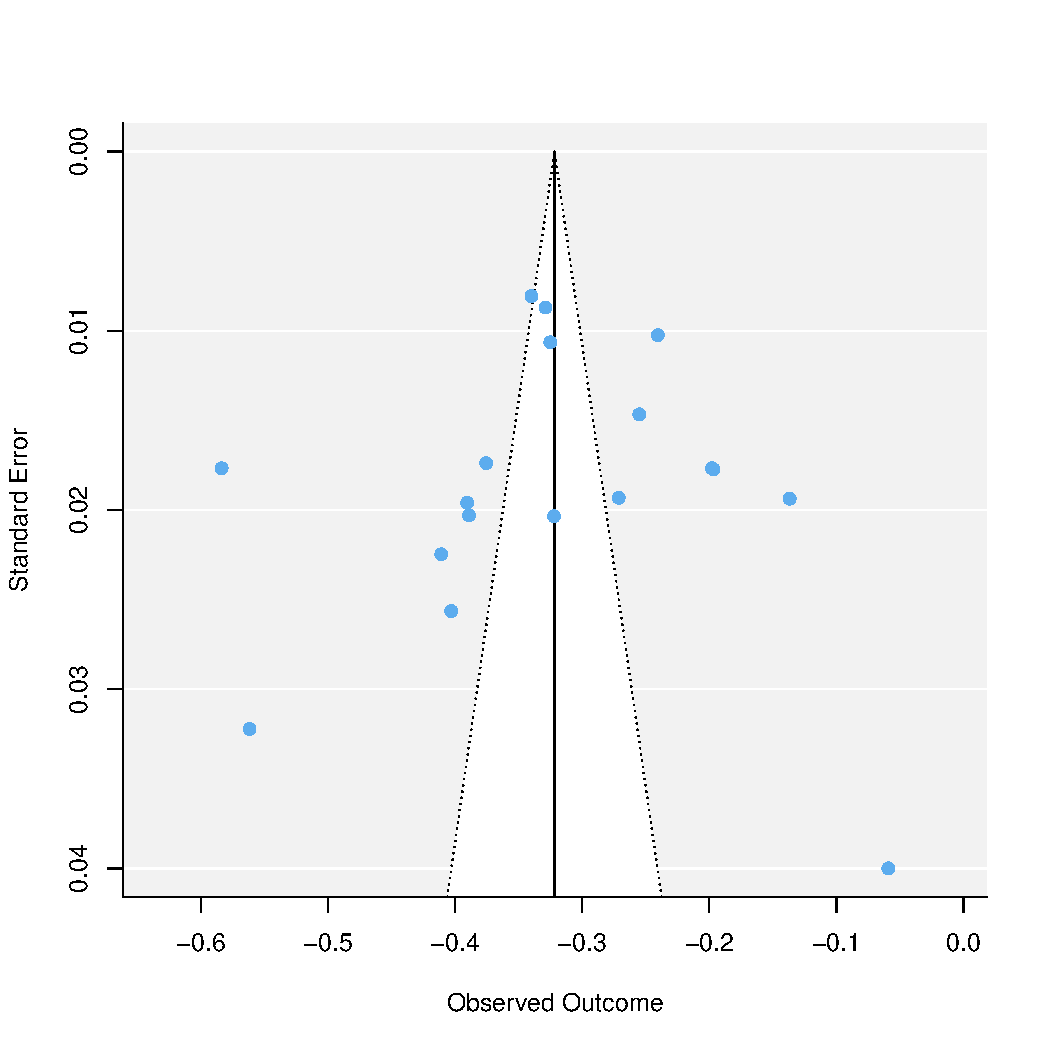
\includegraphics[scale=0.57]{../figs/funnel_re_survey.pdf}
\vspace{0.2cm}
\caption{Funnel plot: survey experiments}.
\small
\vspace{-0.3cm}
\label{fig: funnel_re_survey}
\end{centering}
\end{figure}

\begin{figure}[!htb]
\begin{centering}
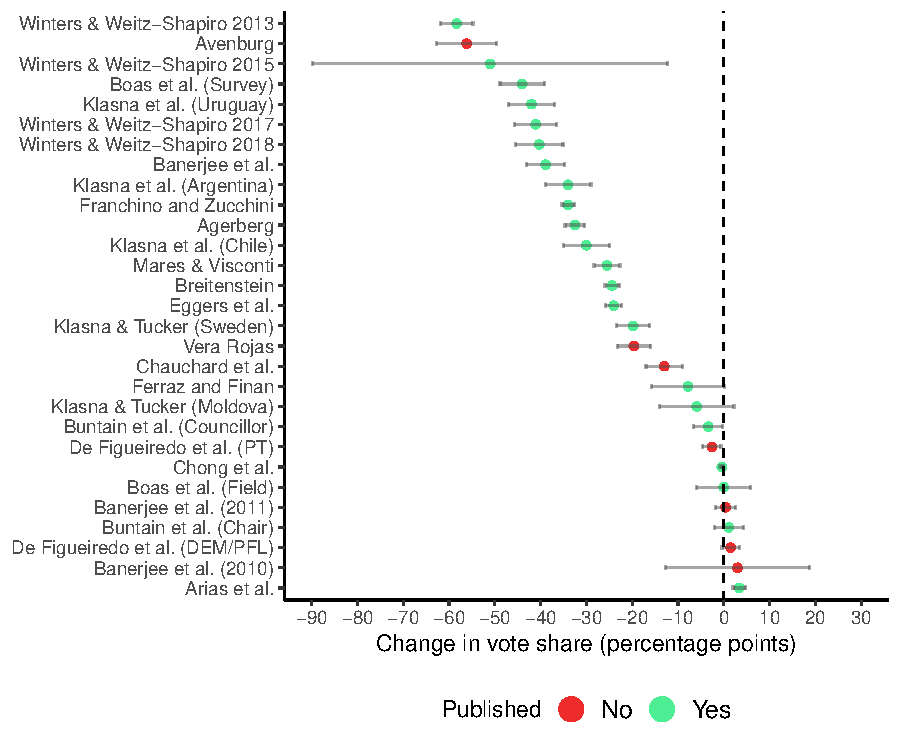
\includegraphics[scale=1]{../figs/published.pdf}
\vspace{0.2cm}
\caption{All experiments by publication status: Average treatment effect of corruption information on vote share and 95\% confidence intervals}.
\small
\vspace{-0.3cm}
\label{fig: pub_status_chart}
\end{centering}
\end{figure}

\clearpage
\pagebreak

\subsection{Information quality}

\begin{figure}[!htb]
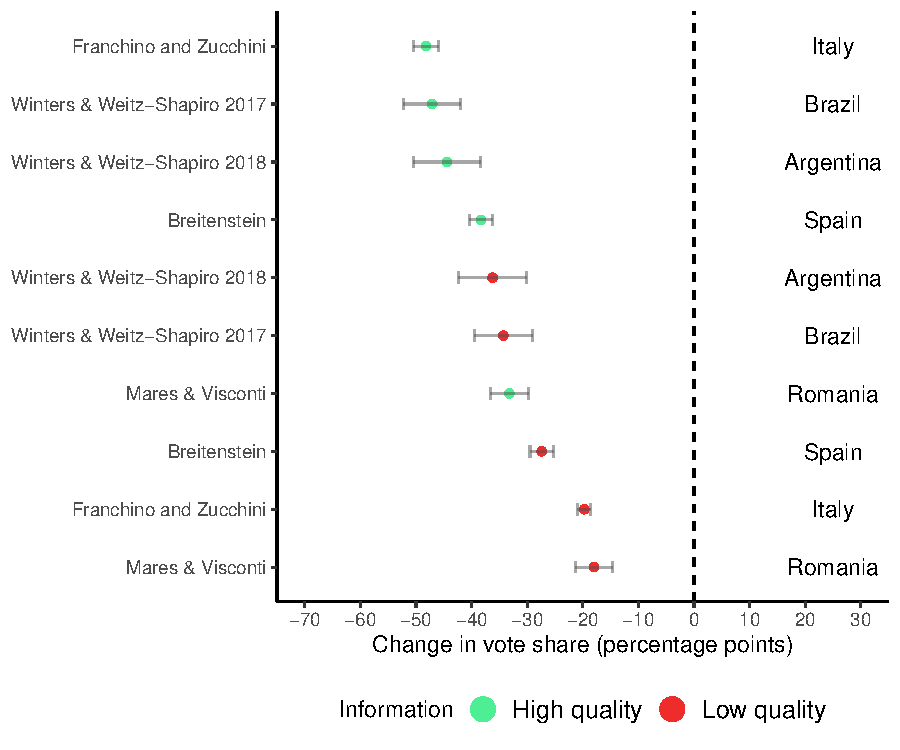
\includegraphics[scale=0.93]{../figs/quality.pdf}
\vspace{0.2cm}
\caption{Survey experiments by information quality: Average treatment effect of corruption information on vote share and 95\% confidence intervals}.
\small
\vspace{-0.3cm}
\label{fig: quality}
\end{figure}

\clearpage
\pagebreak

\subsection{Additional conjoint replications using predicted probabilities}

\subsubsection{\citet{breitenstein2019choosing}}

\begin{figure}[!htb]
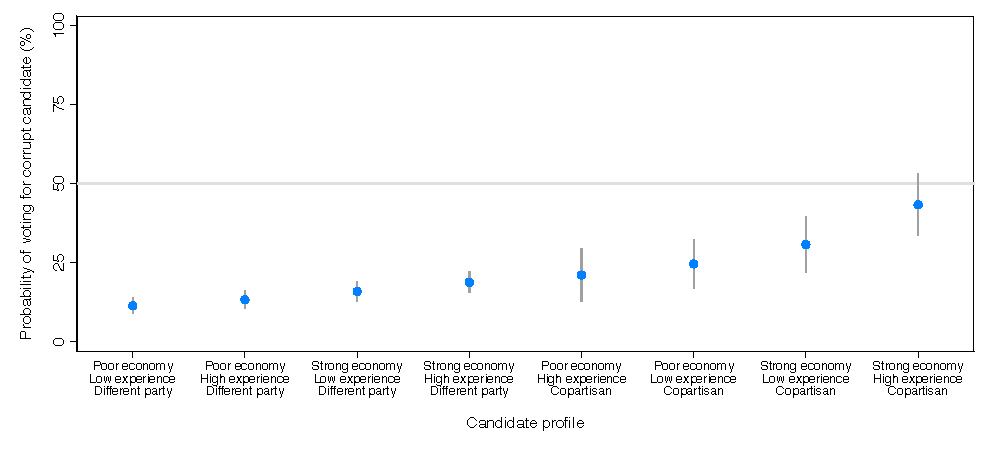
\includegraphics{../figs/b_margins_clean.pdf}
\vspace{0.05cm}
\caption{\citet{breitenstein2019choosing} conjoint: can the right candidate overcome corruption (clean challenger)?}
\small
\vspace{-0.5cm}
\label{fig: b_margins_clean}
\end{figure}

\begin{figure}[!htb]
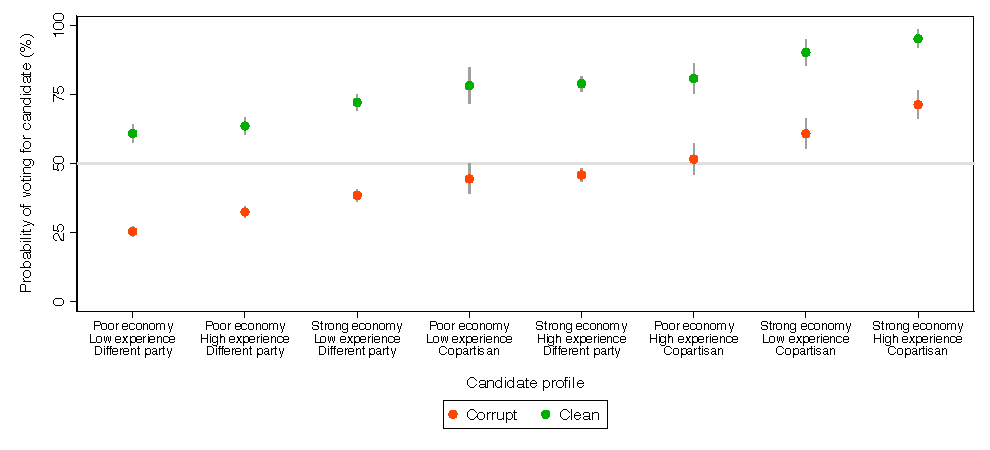
\includegraphics{../figs/b_margins_corrupt_clean.pdf}
\vspace{0.05cm}
\caption{\citet{breitenstein2019choosing} conjoint: probability of choosing candidate (by clean or corrupt)}
\small
\vspace{-0.5cm}
\label{fig: b_margins_corrupt_clean}
\end{figure}

\begin{figure}[!ht]
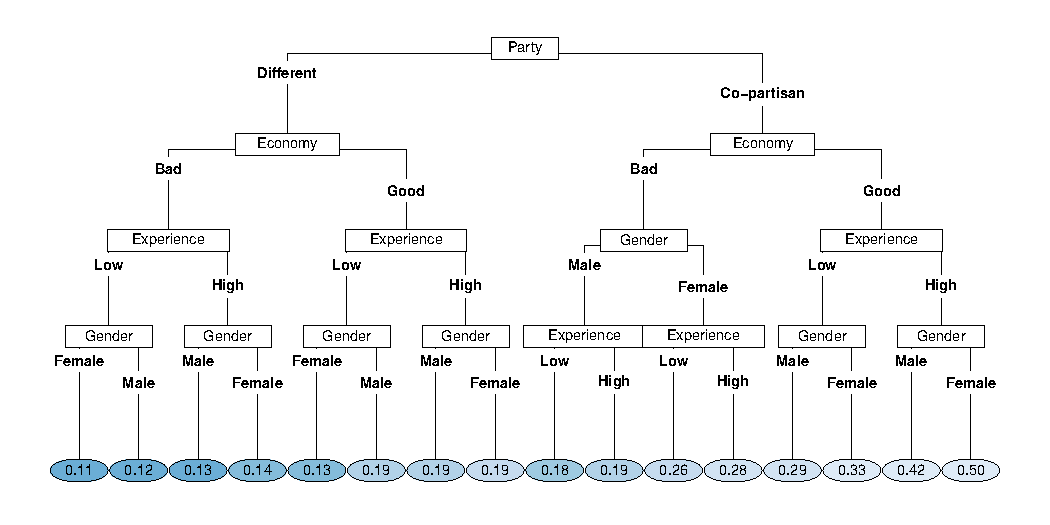
\includegraphics{../figs/b_tree_clean.pdf}
\vspace{-0.5cm}
\caption{\citet{breitenstein2019choosing} conjoint decision tree: predicted probabilities of voting for corrupt politician with clean challenger}
\small
\label{fig: b_tree_clean}
\end{figure}


\clearpage
\pagebreak

\subsubsection{\citet{franchino2015voting}}

\begin{figure}[!htb]
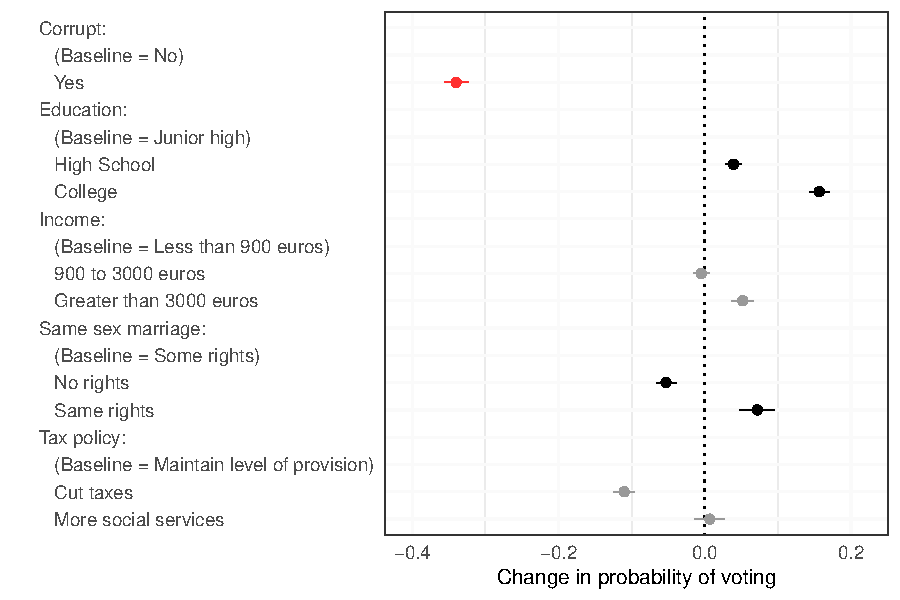
\includegraphics{../figs/fz_amce.pdf}
\caption{\citet{franchino2015voting} conjoint: AMCEs}
\label{fig: fz_amce}
\end{figure}


\begin{figure}[!htb]
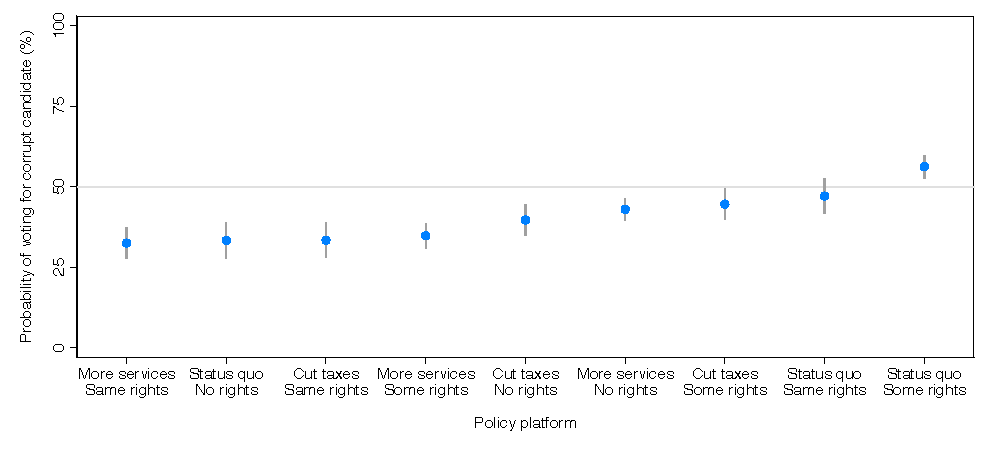
\includegraphics{../figs/fz_margins_right.pdf}
\vspace{0.2cm}
\caption{\citet{franchino2015voting} conjoint: can policy positions overcome corruption (conservative respondents)?}
\small
\vspace{-0.3cm}
\label{fig: fz_margins_right}

\vspace{1cm}

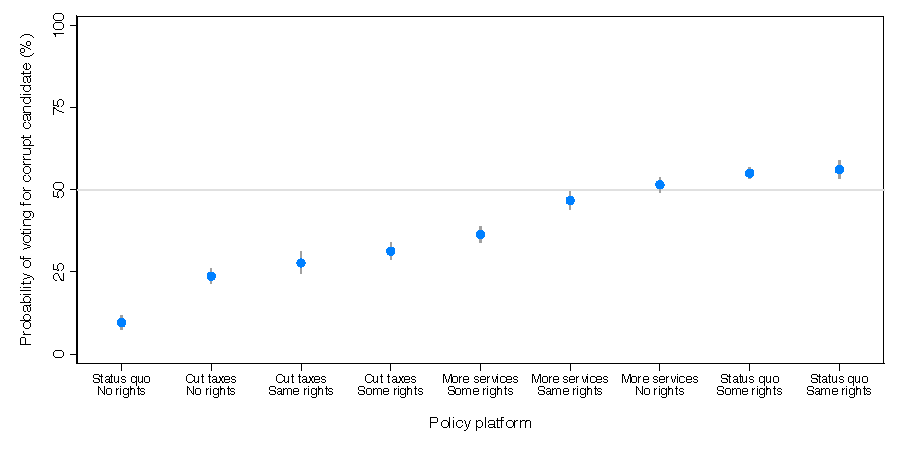
\includegraphics{../figs/fz_margins_left.pdf}
\vspace{0.2cm}
\caption{\citet{franchino2015voting} conjoint: can policy positions overcome corruption (liberal respondents)?}
\small
\vspace{-0.3cm}
\label{fig: fz_margins_left}
\end{figure}

\begin{figure}[!htb]
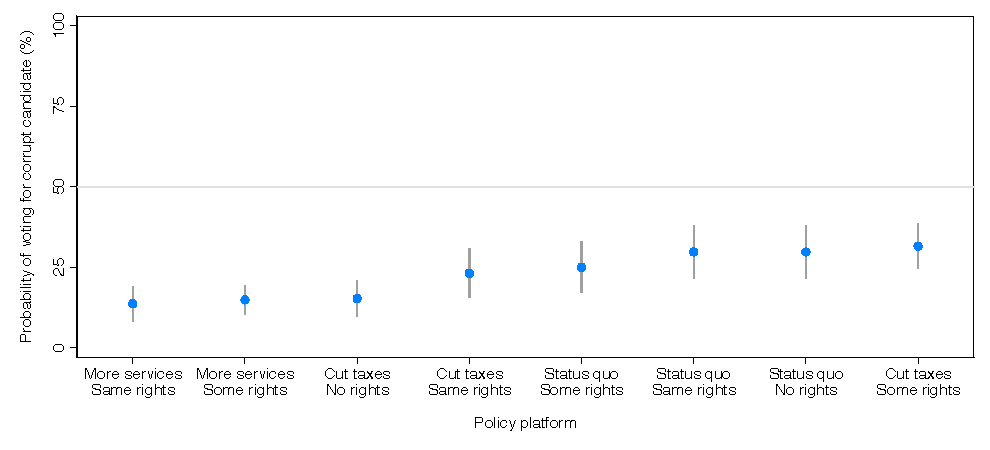
\includegraphics{../figs/fz_margins_right_clean.pdf}
\vspace{0.2cm}
\caption{\citet{franchino2015voting} conjoint: can policy positions overcome corruption (conservative respondents and clean challenger)?}
\small
\vspace{-0.3cm}
\label{fig: fz_margins_right_clean}

\vspace{1cm}

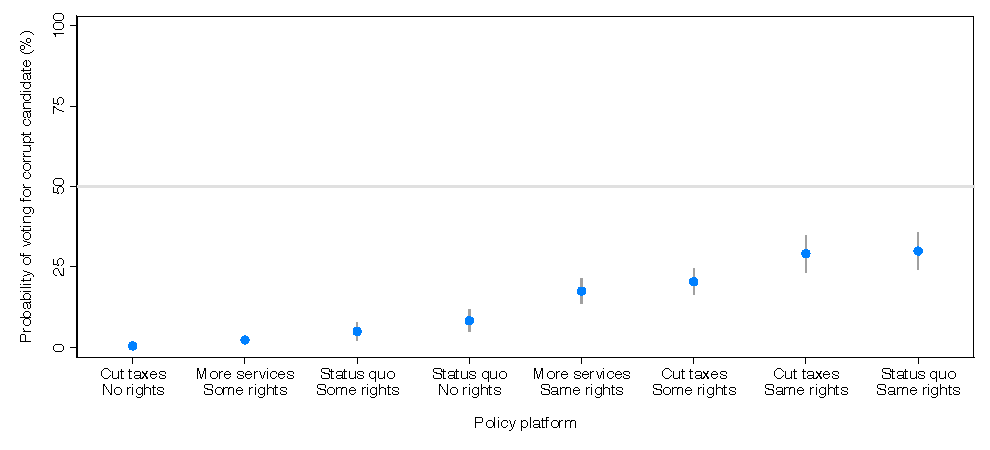
\includegraphics{../figs/fz_margins_left_clean.pdf}
\vspace{0.2cm}
\caption{\citet{franchino2015voting} conjoint: can policy positions overcome corruption (liberal respondents and clean challenger)?}
\small
\vspace{-0.3cm}
\label{fig: fz_margins_left_clean}
\end{figure}

\clearpage
\pagebreak

\subsubsection{\citet{mares2019voting}}

\begin{figure}[!htb]
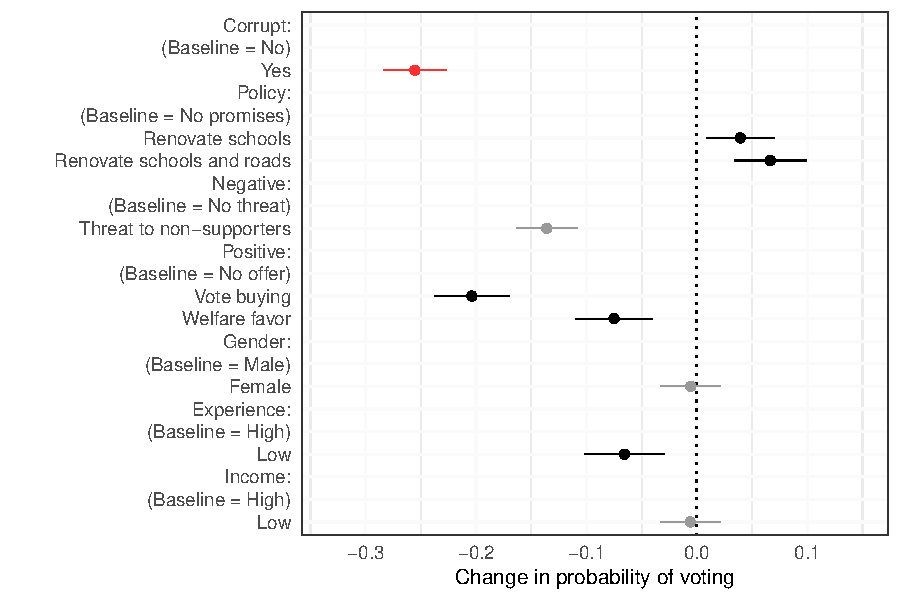
\includegraphics{../figs/mv_amce.pdf}
\caption{\citet{mares2019voting} conjoint: AMCEs}
\label{fig: mv_amce}
\end{figure}

\begin{figure}[!htb]
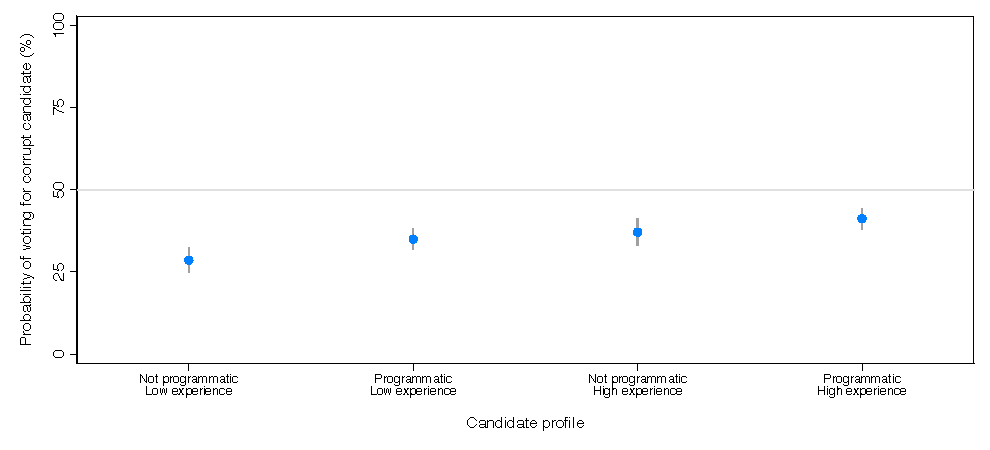
\includegraphics{../figs/mv_margins.pdf}
\vspace{0.2cm}
\caption{\citet{mares2019voting} conjoint: can programmatic offerings and experience overcome corruption?}
\small
\vspace{-0.3cm}
\label{fig: mv_margins}
\end{figure}

\noindent
\normalsize	
Note that the primary goal of \citet{mares2019voting} is to determine the degree to which respondents punish various illicit electoral activities. The experiment therefore includes a number of other negative attributes in addition to corruption, such as vote buying, clientelistic offerings, and threats of violence against political opponents.  Due to uniform randomization, calculating predicted probabilities that do not include these attributes therefore marginalizes over a number of other illicit activities that respondents view negatively and reduces overall vote probability. Conditioning on the candidate not engaging in illicit activities other than corruption reveals probabilities of voting for corrupt candidates over 50\%. 

\begin{figure}[!htb]
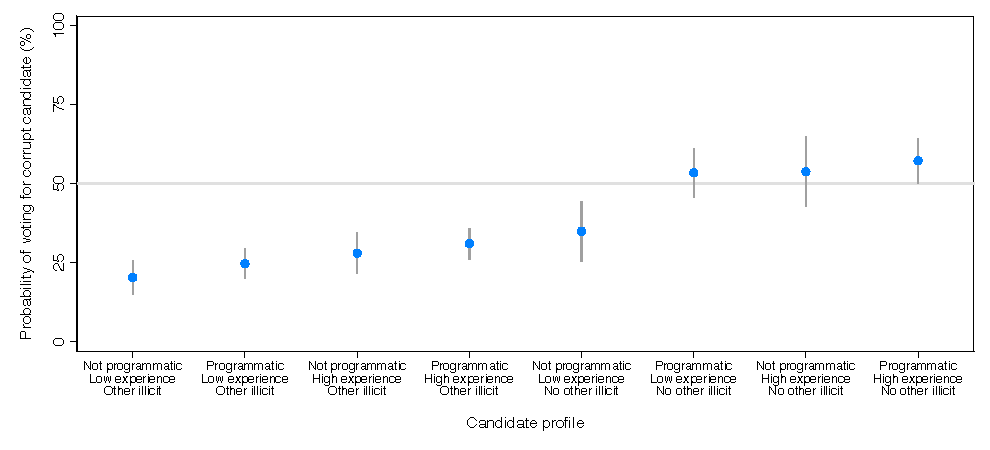
\includegraphics{../figs/mv_margins_illicit.pdf}
\vspace{0.2cm}
\caption{\citet{mares2019voting} conjoint: can programmatic offerings and experience overcome corruption (conditional on other illicit activities)?}
\small
\vspace{-0.3cm}
\label{fig: mv_margins_illicit}
\end{figure}

\clearpage
\pagebreak

\subsubsection{\citet{chauchard2019getting}}

%\begin{figure}[!htb]
%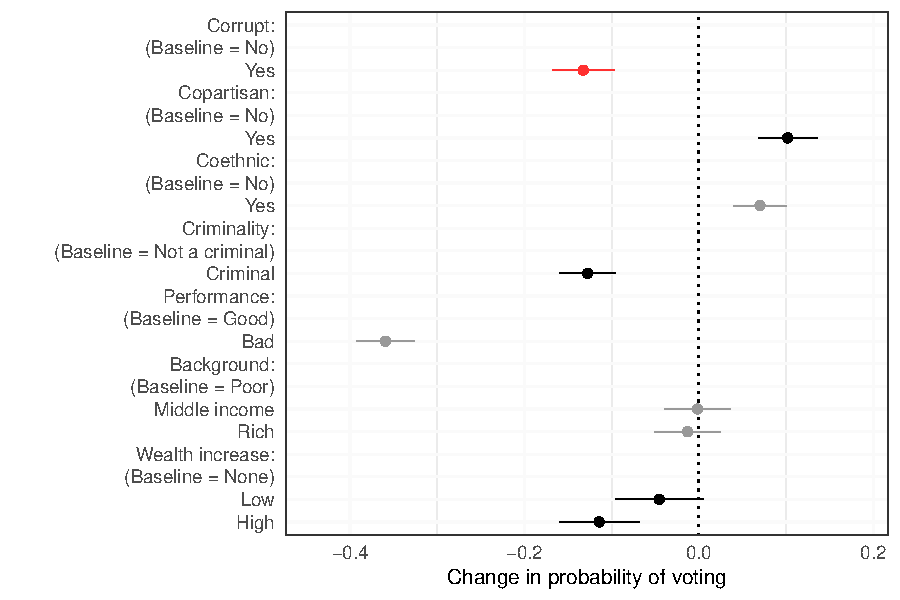
\includegraphics{../figs/ckh_amce.pdf}
%\caption{\citet{chauchard2019getting} conjoint: AMCEs}
%\label{fig: ckh_amce}
%\end{figure}

\begin{figure}[!htb]
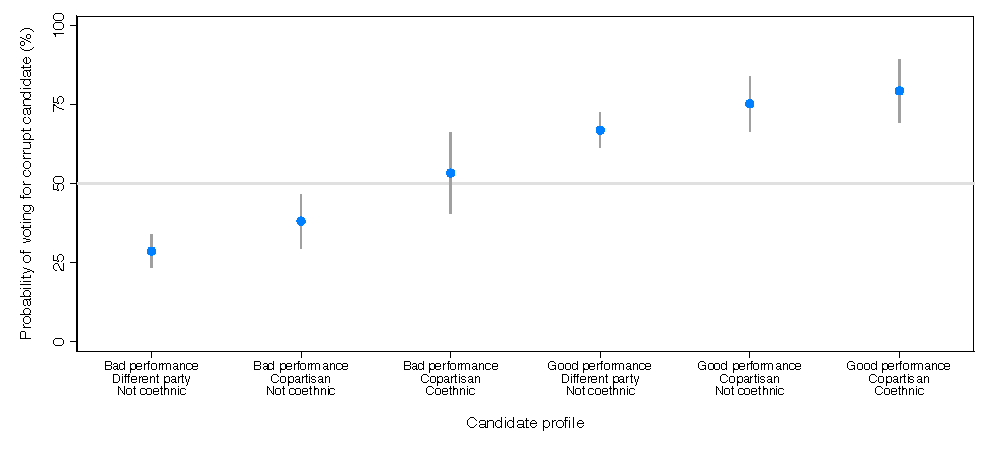
\includegraphics{../figs/ckh_margins.pdf}
\vspace{0.2cm}
\caption{\citet{chauchard2019getting} conjoint: can performance, partisanship, and coethnicity overcome corruption?}
\small
\vspace{-0.3cm}
\label{fig: ckh_margins}
\end{figure}

\begin{figure}[!ht]
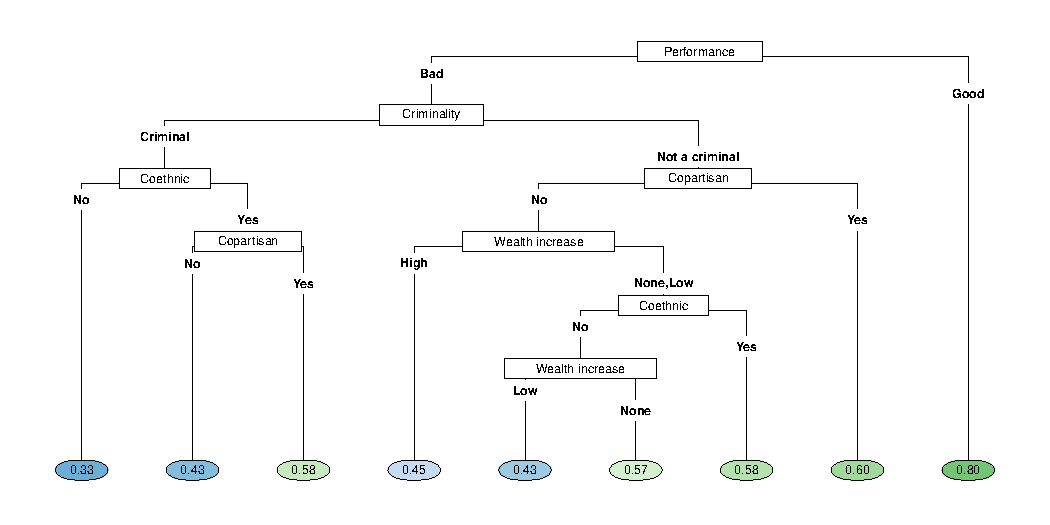
\includegraphics{../figs/ckh_tree_corrupt.pdf}
\vspace{-0.5cm}
\caption{\citet{chauchard2019getting} conjoint decision tree: predicted probabilities of voting for corrupt politician}
\small
\label{fig: b_tree_clean}
\end{figure}

\clearpage
\FloatBarrier


\end{document} 